\chapter{当代扩散模型：分数SDE框架}\label{ch:score-sde}

\epigraph{
    \textit{只有一种精确的方式来表达这些定律，那就是通过微分方程。它们的优点是基础性强，并且据我们所知，是精确的。
}}{理查德·费曼}



前两章分别介绍了扩散模型的变分视角和源于能量模型的分数视角。本章把时间推广到连续情形，用\emph{分数 SDE}~\citep{song2020score}在同一个框架中描述 DDPM 与 NCSN。

可以想象在数据与噪声之间不断插入更多中间噪声水平。在连续时间极限下，噪声水平随时间平滑变化，前向和反向过程可写为
\[
    p_{\mathrm{data}}
    \;\xrightarrow{\text{forward SDE}}\;
    p_T \approx p_{\mathrm{prior}},
    \qquad
    p_{\mathrm{prior}}
    \;\xrightarrow{\text{reverse dynamics}}\;
    p_{\mathrm{data}}.
\]
前向 SDE 描述了数据如何逐渐损坏为噪声，播放
DDPM 中噪声表的连续时间作用或噪声序列
NCSN 级别。一旦指定了这个前向过程，主要的挑战是
相反方向的生成：从简单的噪声分布开始，
我们如何恢复数据分布？

关键数量是与时间相关的分数
\[
    \nabla_{\rvx}\log p_t(\rvx),
\]
它描述了每次噪声分布的局部几何形状
$t$。一旦知道这个分数，或者通过神经网络近似，它就可以确定用于生成的逆时动态，将噪声转换为数据。这导致两个互补的
描述：随机 \emph{ 反向时间 SDE} 和确定性
\emph{ 概率流 ODE} (PF-ODE)。尽管他们的样本轨迹是
不同的是，它们可以遵循相同的边缘分布演化。

这种连续时间视图将生成问题转变为解决问题
微分方程，为随机性的一系列广泛工具打开了大门
过程、微分方程和数值分析。特别是有一次
生成动力学被写成 SDE 或 ODE，标准数值
可以使用方法来模拟它们，而更高级的求解器可以改进
采样效率和准确性。因此，这一观点不仅提供了
扩散模型的统一数学描述，也是一种实用的
为理解和设计更快的采样方法奠定了基础
本书稍后会介绍。\chapterlearning{
  \item 了解DDPM和NCSN的离散噪声水平如何导致连续时间前向SDE逐渐将数据转化为噪声；
  \item 了解如何通过随机反向时间 SDE 或确定性概率流 ODE (PF-ODE) 来描述从噪声生成数据的过程；
  \item 解释反向时间 SDE 和 PF-ODE 如何在各自样本轨迹不同的情况下遵循相同的边缘分布序列，并理解 福克尔-普朗克方程如何描述概率密度的连续时间演化；
  \item 了解如何通过去噪分数匹配来学习时间相关分数，然后通过反向时间 SDE 或 PF-ODE 用于采样；
  \item 了解PF-ODE如何也可以向前运行进行反演，并通过变量的连续变化公式跟踪概率密度的变化，从而实现似然评估；
  \item 将 VE 和 VP SDE 视为同一连续时间扩散框架的两个重要实例，连接回 NCSN 和 DDPM。
}{
刚接触随机微分方程的读者可以根据需要查阅\Cref{app:de}中的微分方程附录。对于第一遍，重点关注正向 SDE、反向时间 SDE 和 PF-ODE 的角色，以及它们的训练和采样程序。在主图清晰之后，可以重新审视高斯示例和可选推导。
}




























































    

























































\newpage

\section{分数 SDE 的原理}\label{sec:dm-today}


\begin{figure}[th!]
    \centering
    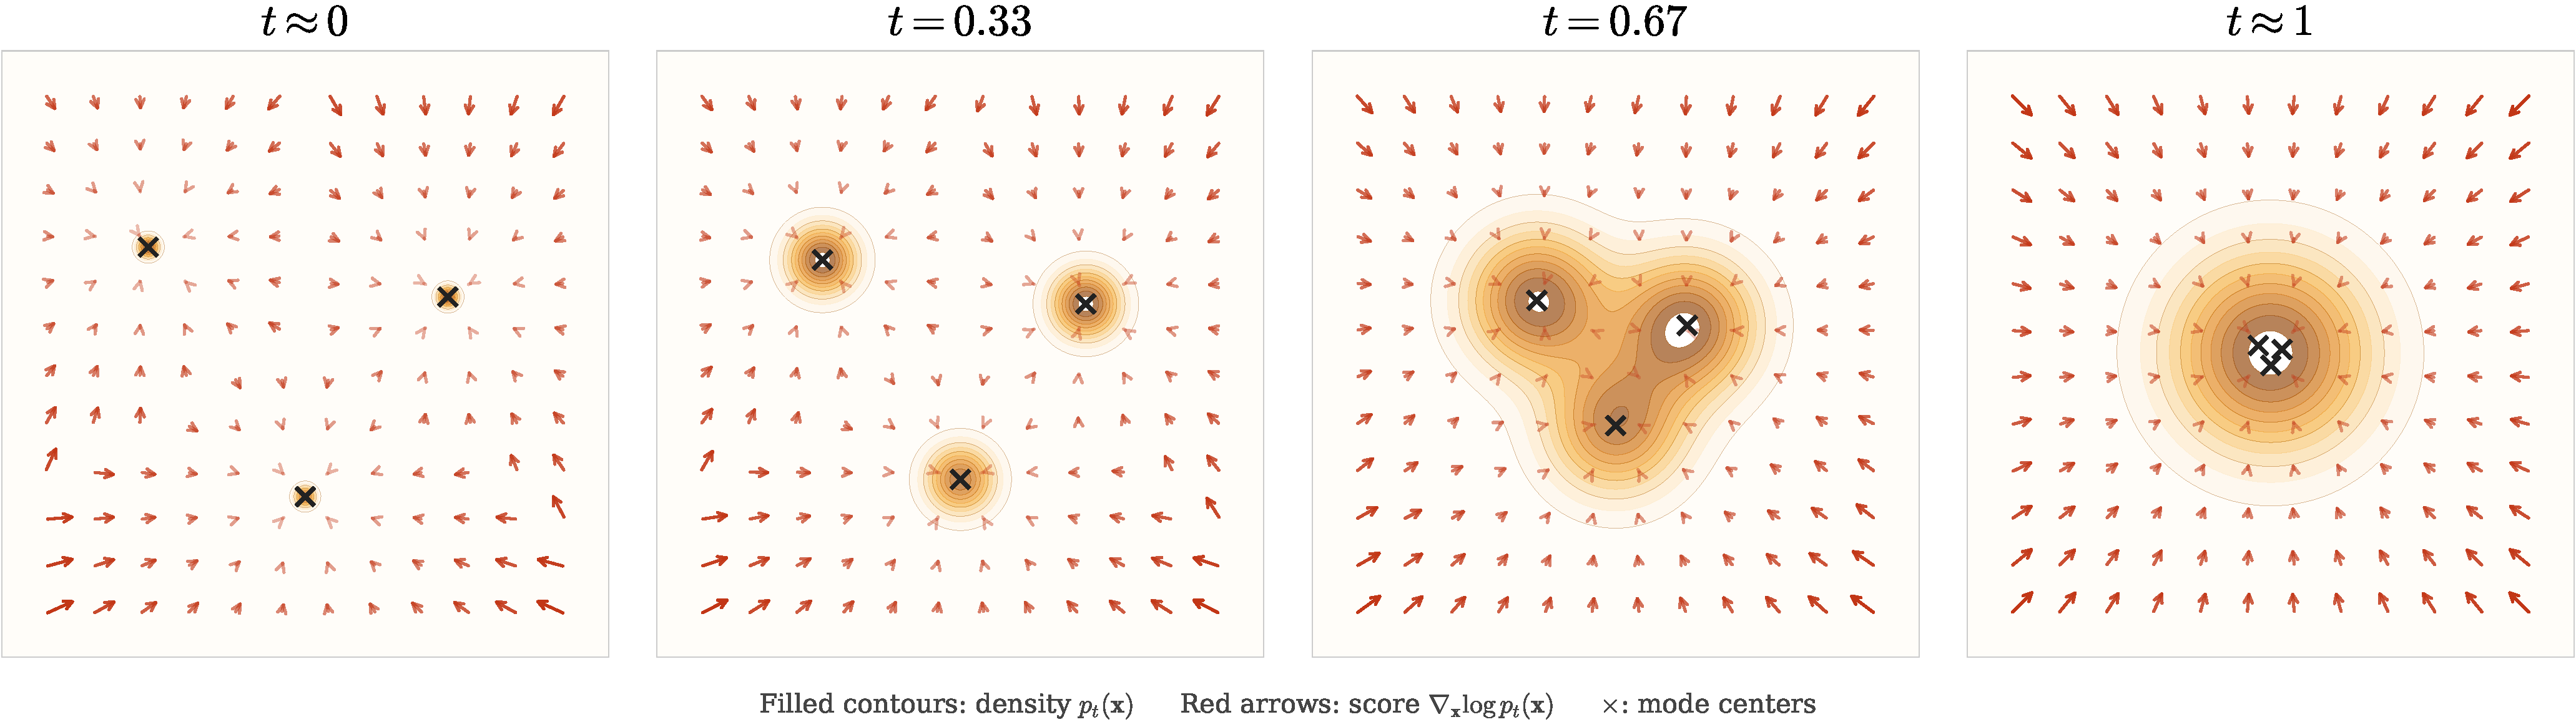
\includegraphics[width=\linewidth]{Images/PartB/score_landscape_2d.pdf}
    \caption{\textbfs{ 时间相关分数景观的图示。}
随着噪声水平的增加，扰动密度 $p_t(\rvx)$ 从集中在数据模式附近的多峰分布（数据）演变为广泛的近单峰分布（先前）。
因此，分数场 $\nabla_{\rvx}\log p_t(\rvx)$ 从将样本拉向附近模式的尖锐局部矢量场变为指向整体质心的平滑全局场。
这个与时间相关的分数字段是基于分数的扩散模型（即分数 SDE）中学习的关键对象。 \figcredit{由作者使用AI辅助编码创建。}}
    \label{fig:time-dependent-score}
\end{figure}

多种噪声尺度的使用是 NCSN 和 DDPM 框架成功的关键因素。在本节中，我们将介绍该框架的基础 \emph{分数 SDE}~\citep{song2020score}，它通过考虑连续的噪声水平来提升这个想法。正向和反向扩散过程的连续时间极限已经被注意到 \citet{sohl2015deep}，但是 \citet{song2020score} 通过将数据演化公式化为随机/常微分方程，使这一观点成为中心，其中噪声水平随着时间的推移平稳增加。这个公式的核心是 \emph{与时间相关的分数函数} $\nabla_{\rvx}\log p_t(\rvx)$: 在每个噪声级别~$t$，它指向当前噪声分布下密度较高的区域~$p_t$，正是这个量决定了如何反转扩散。作为 \Cref{fig:time-dependent-score} 说明，分数场从急剧收敛到小的个体数据模式演变~$t$ 轻轻地指向整个全球中心~$t$。这种连续时间公式不仅统一了先前的离散时间模型，而且还为生成建模提供了有原则且灵活的基础：在所有噪声级别上学习这一系列分数函数可以减少求解微分方程问题的生成。









\subsection{动机：从离散过程到连续时间过程}\label{subsec:scoresde-motivation}


我们重新审视 NCSN 和 DDPM 的前向噪声注入方案。 NCSN 使用一系列逐渐增加的噪声级别 $\{\sigma_i\}_{i=1}^L$。每个干净的样品 $\rvx_0 \sim p_{\mathrm{data}}$ 被扰乱为
\[
\rvx_{\sigma_i} = \rvx_0 + \sigma_i \bm{\epsilon}_i, 
\qquad \bm{\epsilon}_i \sim \mathcal{N}(\bm{0}, \rmI).
\]
DDPM 使用方差计划增量注入噪声 $\{\beta_i\}_{i=1}^L$\footnote{在 \Cref{sec:ddpm}，DDPM前向步长写为 $\rvx_i = \sqrt{1-\beta_i^2}\,\rvx_{i-1} + \beta_i\,\bm{\epsilon}_i$，其中 $\beta_i$ 表示注入噪声的标准偏差 $\alpha_i := \sqrt{1-\beta_i^2}$。在这里以及本章中，我们遵循以下约定： \citet{song2020score}，其中 $\beta_i$ 而是表示注入噪声的方差，因此 $\rvx_i = \sqrt{1-\beta_i}\,\rvx_{i-1} + \sqrt{\beta_i}\,\bm{\epsilon}_i$。这两个约定的关系是 $\beta_i^{\textup{(here)}} = \bigl(\beta_i^{\textup{(Ch.\ \ref{ch:variational})}}\bigr)^2$ 并产生相同的动态。}:
\[
\rvx_i = \sqrt{1 - \beta_i}\, \rvx_{i-1} + \sqrt{\beta_i}\, \bm{\epsilon}_i, 
\qquad \bm{\epsilon}_i \sim \mathcal{N}(\bm{0}, \rmI).
\]

我们在离散时间网格上一起查看它们，其中的顺序更新 $\rvx_t$ 至 $\rvx_{t+\Delta t}$ 采用以下形式\footnote{为了方便起见，我们使用 $\rvx(t)$ 和 $\rvx_t$ 可互换（对于其他随时间变化的变量类似）以表示时间样本 $t$.}:
\begin{align*}
    \text{\textbfs{NCSN:}} \,\,
    & \rvx_{t+\Delta t} = \rvx_t + \sqrt{\sigma_{t+\Delta t}^2 - \sigma_t^2} \bm{\epsilon}_t 
    &&\approx \rvx_t + \sqrt{\frac{\diff \sigma_t^2}{\diff t} \Delta t}  \bm{\epsilon}_t \\[0.5em]
    \text{\textbfs{DDPM:}} \,\,
    & \rvx_{t+\Delta t} = \sqrt{1 - \beta(t)\Delta t} \rvx_t + \sqrt{\beta(t)\Delta t} \bm{\epsilon}_t 
    &&\approx \rvx_t - \frac{1}{2} \beta(t) \rvx_t  \Delta t + \sqrt{\beta(t)\Delta t}  \bm{\epsilon}_t,
\end{align*}
其中 $\bm{\epsilon}_t \sim \mathcal{N}(\bm{0}, \rmI)$。有趣的是，两种噪声注入过程都遵循共同的结构模式：
\begin{align}\label{eq:euler-discrete-sde}
    \rvx_{t+\Delta t} \approx \rvx_t + \rvf(\rvx_t, t) \Delta t + g(t) \sqrt{\Delta t}\, \bm{\epsilon}_t,
\end{align}
与 $\rvf: \mathbb{R}^D \times \mathbb{R} \to \mathbb{R}^D$ 和 $g: \mathbb{R} \to \mathbb{R}$ 由以下公式给出：
\begin{align*}
    \text{\textbfs{NCSN:}} \quad 
    & \rvf(\rvx, t) = 0, \qquad g(t) = \sqrt{\frac{\diff \sigma^2(t)}{\diff t}} \\[0.5em]
    \text{\textbfs{DDPM:}} \quad 
    & \rvf(\rvx, t) = -\frac{1}{2} \beta(t)\, \rvx, \qquad g(t) = \sqrt{\beta(t)}.
\end{align*}


\begin{figure}
    \centering
    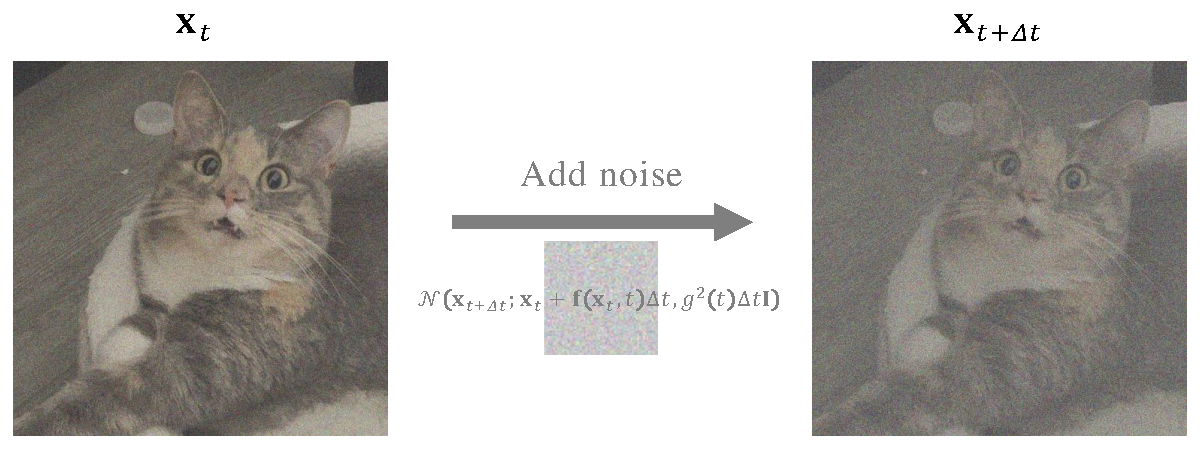
\includegraphics[width=0.9\linewidth]{Images/PartB/sde-forward-noise.pdf}
    \caption{\textbfs{离散时间噪声添加步骤的图示。} 它增加了来自 $t$ 至 $t + \Delta t$ 带平均漂移 $\rvf(\rvx_t, t)$ 和扩散系数 $g(t)$. \figcredit{由作者创建。}}
    \label{fig:sde-forward-noise}
\end{figure}该公式对应于以下高斯跃迁：
\begin{align}\label{eq:transition-forward-f-g}
    p(\rvx_{t+\Delta t} |\rvx_t) := \mathcal{N}\!\left(\rvx_{t+\Delta t}; \rvx_t + \rvf(\rvx_t, t)\Delta t,\, g^2(t)\Delta t\, \rmI\right),
\end{align}
其中，由于符号的轻微滥用，我们将 $\rvx_t$ 视为固定样本，将 $\rvx_{t+\Delta t}$ 视为随机变量。

作为$\Delta t \to 0$（概念上可以理解为准备\emph{无穷多个}噪声层），离散时间过程收敛到在时间上向前演化的连续时间SDE\footnote{\Cref{eq:transition-forward-f-g}中的前向转移核收敛为$\Delta t\to0$，解为相应的Itô SDE。完全严格的证明依赖于我们遵循文献的先进结果。}：
\begin{align*}
    \diff \rvx(t) = \rvf(\rvx(t), t) \diff t + g(t) \diff \rvw(t),
\end{align*}
其中 $\rvw(t)$ 是标准维纳过程（或布朗运动）。
\rmkb{虽然这里不需要完整的正式定义，但 \emph{ 维纳过程 } 是一个连续时间随机过程 $ \rvw(t) $，它从零开始，具有独立增量，并且满足对于任何 $ s < t $，增量 $ \rvw(t) - \rvw(s) $ 服从均值为零的正态分布和方差 $ t - s $。它代表独立高斯波动随时间的累积，虽然它几乎肯定是连续的，但它是不可微分的。

在无穷小的时间间隔 $[t, t + \diff t]$ 上，维纳过程的增量定义为
\[
\diff \rvw(t) := \rvw(t + \diff t) - \rvw(t),
\]
其被建模为均值和方差为零的高斯随机变量 $\diff t$：
\[
\diff \rvw(t) \sim \mathcal{N}(\bm{0}, \diff t \rmI).
\]}

\Cref{app:sde-intro} 中提供了对 SDE 基础的简要介绍，\Cref{app:Ito} 中提供了更高级的讨论。然而，我们可以从概念上理解离散公式和连续公式之间的联系如下：
\begin{itemize}
    \item $\rvx(t+\Delta t) - \rvx(t) \approx \diff \rvx(t)$，
    \item $\Delta t \approx \diff t$，
    \item $\sqrt{\Delta t} \bm{\epsilon}_t \sim \mathcal{N}(\bm{0}, \Delta t \rmI) \approx \diff \rvw(t)$。
\end{itemize}
一旦指定了漂移 $\rvf(\rvx,t)$ 和扩散 $g(t)$，正向时间 SDE 就会自动引发反向时间 SDE，将终端噪声分布传输回数据分布。反向动态仅涉及单个未知项，令人惊讶的是每个连续时间级别的 \emph{score 函数 }。这将分数匹配确定为训练目标；一旦学习到分数，采样就相当于将反向时间 SDE 与学习到的分数进行数值积分。


虽然 \Cref{sec:scoresde-training-sampling} 提出了实际实现，但我们首先研究了 \Cref{subsec:forward-sde} 和 \Cref{subsec:reverse-sde} 中正向和反向过程的理论基础。

\subsection{正向时间 SDE：从数据到噪声}\label{subsec:forward-sde}
\begin{figure}[th!]
    \centering
    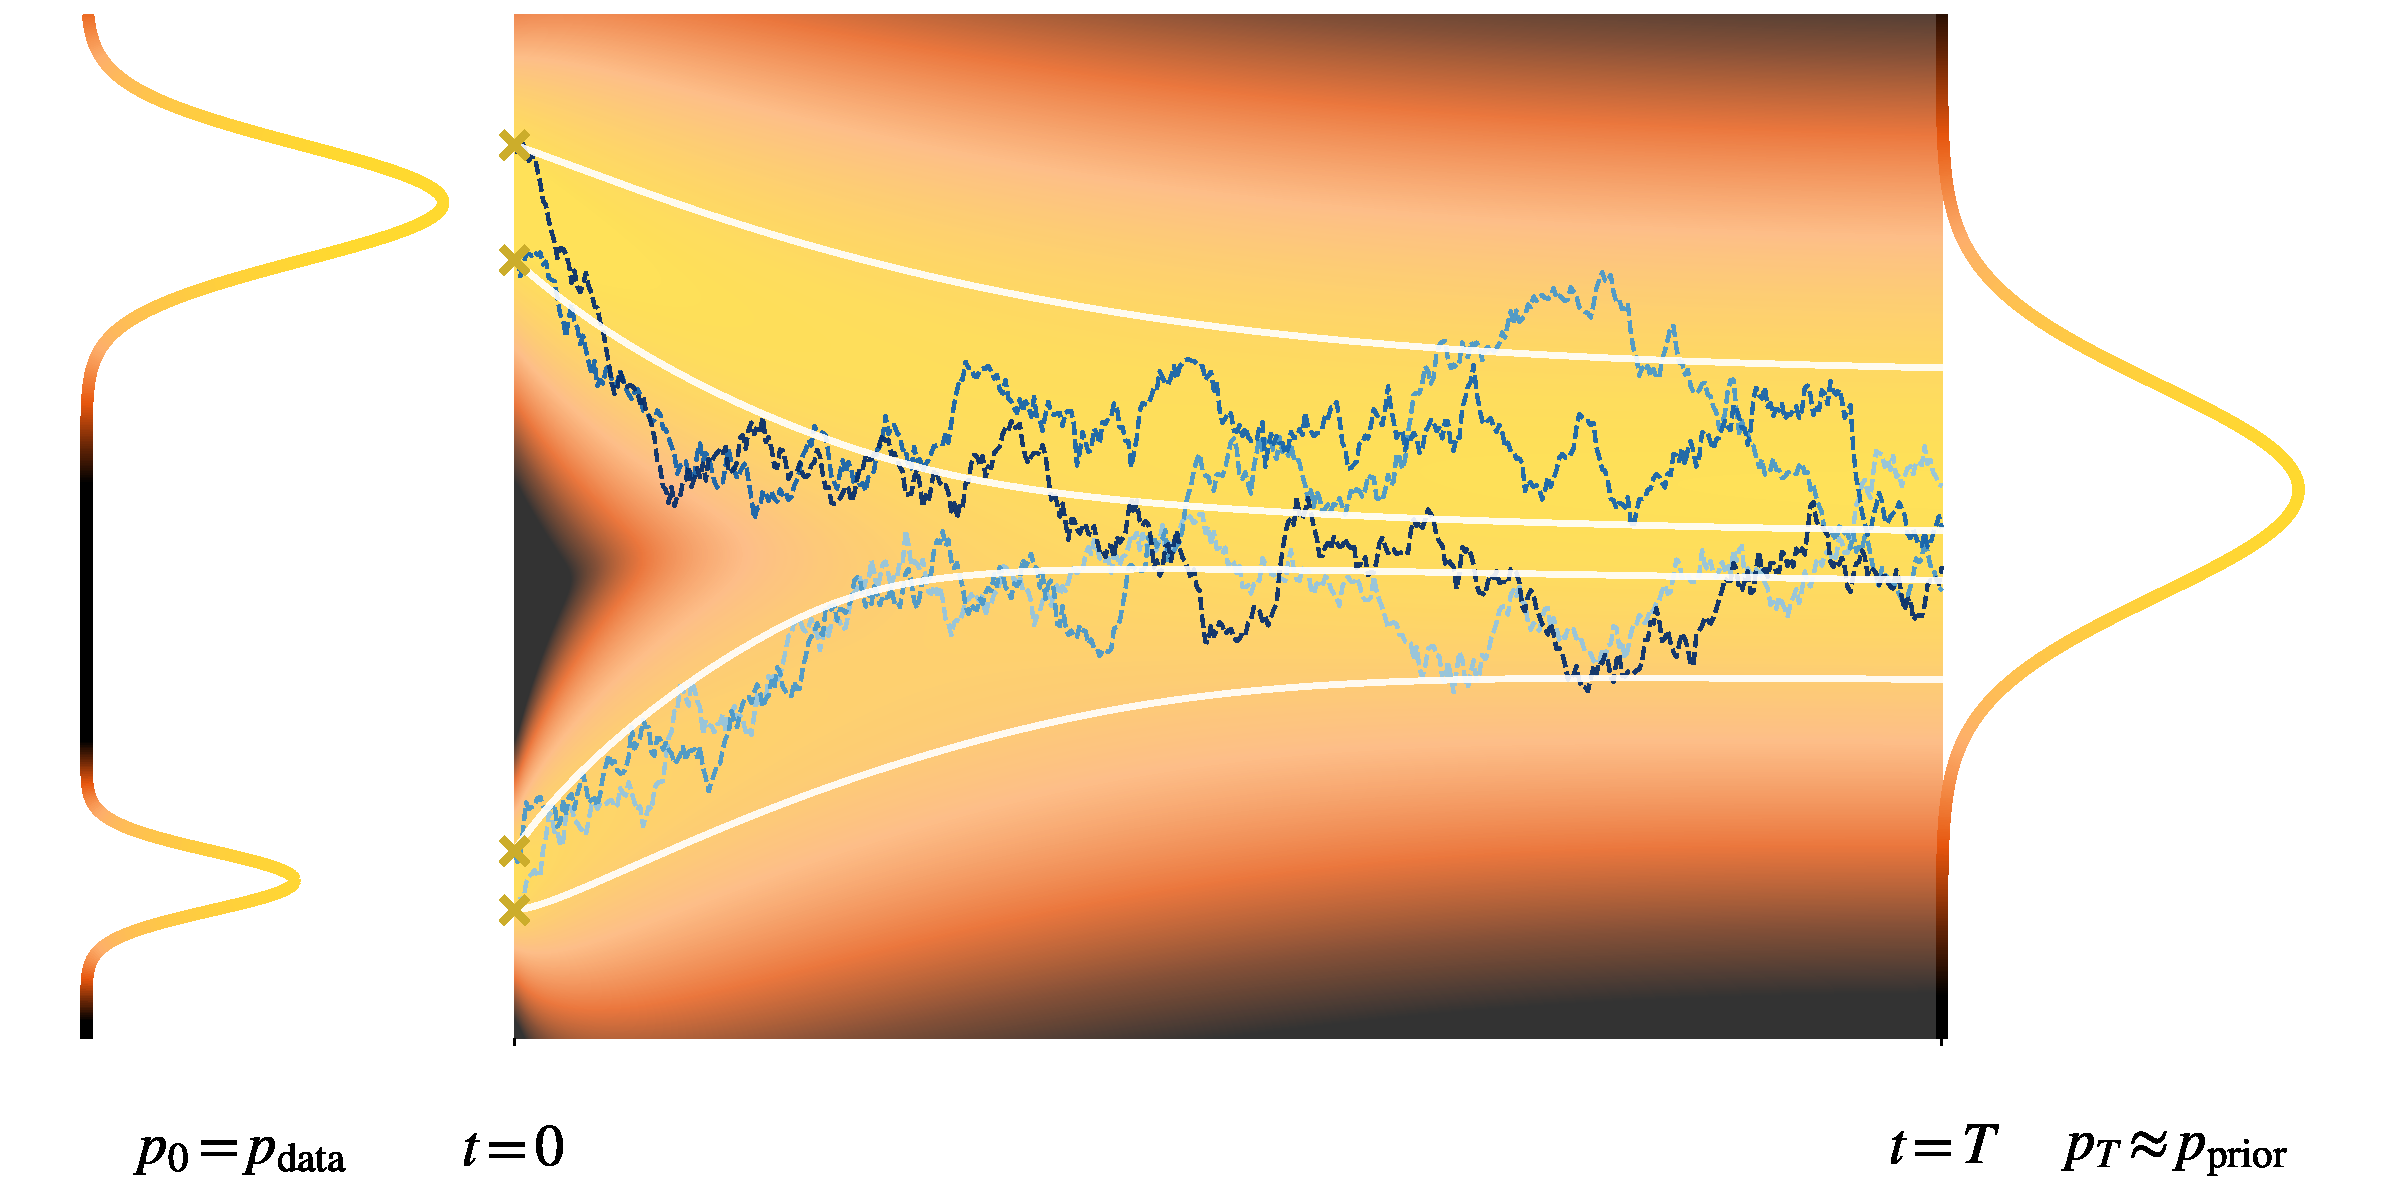
\includegraphics[width=\textwidth]{Images/PartB/forward_sde_ode_trajectories.pdf}
        \caption{\textbfs{(1D) 扩散模型中前向过程的可视化。} 该过程从采样的初始点开始（表示为``$\times$'') 来自复杂的双峰数据分布 ($p_0 = p_{\mathrm{data}}$) 并演化为简单的单峰高斯先验 ($p_T \approx p_{\mathrm{prior}}$）。背景热图说明了不断变化的边缘概率密度， $p_t$，随着时间的推移而平滑。显示了样本轨迹的演变过程 $t=0$ 至 $t=T$将随机前向 SDE 过程（蓝色路径）与其确定性对应过程 PF-ODE（白色路径）进行比较。请注意，PF-ODE 是密度的确定性传输图，通常不是从单点开始的样本路径的平均值。 \figcredit{由作者创建。}}

    \label{fig:sde-density-traj}
\end{figure}


通过这个公式，早期基于离散时间的方法，例如 NCSN~\citep{song2019generative} 和 DDPM~\citep{sohl2015deep,ho2020denoising}，可以统一下 \emph{连续时间} 通过随机过程的框架 $\rvx(t)$ 由间隔上定义的前向 SDE 控制 $[0, T]$:
\begin{mdframed}
\begin{equation}\label{eq:sde_forward}
    \diff\rvx(t) = \mathbf{f}(\rvx(t), t) \diff t + g(t) \diff\rvw(t), \quad \rvx(0) \sim p_{\mathrm{data}}.
\end{equation}
\end{mdframed}
在这里， $\mathbf{f}(\cdot, t)\colon\mathbb{R}^D\to\mathbb{R}^D$ 是漂移， $g(t) \in \mathbb{R}$ 是标量扩散系数，并且 $\rvw(t)$ 表示标准维纳过程。我们将此称为 \emph{转发SDE}，它描述了干净的数据如何随着时间的推移逐渐被扰动为噪声。一旦漂移 $\mathbf{f}$ 和扩散系数 $g$ 已指定，前向过程已完全确定，描述了数据变量如何通过高斯噪声的注入逐渐损坏。特别是，诱导了两个随时间变化的密度族：
\paragraph{扰动核。} 
条件法
\[
p_t(\rvx_t |\rvx_0)
\]
描述如何清理数据样本 $ \rvx_0 \sim p_{\mathrm{data}} $ 演变成其嘈杂的对应物 $\rvx_t$ 当时 $t$。一般来说，漂移项 $\rvf(\rvx,t)$ 在 \Cref{eq:sde_forward} 可以是任意函数 $\rvx$，但一个常见且分析方便的选择是假设它是仿射的：
\begin{equation}\label{eq:affine-drift}
    \rvf(\rvx,t) = f(t) \rvx, 
\end{equation}
其中 $f(t)$ 是标量函数 $t$，通常被视为非正数。在这种结构下，条件过程仍然是高斯给定的
$\rvx_0$，并且扰动核承认通过求解相关均值-方差 ODE 获得的闭式解~\citep{sarkka2019applied}
（另见 \Cref{subsec:scoresde-perturbation-kernel}). {特别是，
\[
p_t(\rvx_t |\rvx_0) = \mathcal{N} \big(\rvx_t; \rvm(t), P(t)\mathbf I_D\big),
\]
有
\[
\rvm(t) = \exp \Big(\int_0^t f(u) \diff u\Big) \rvx_0,
\quad
P(t) = \int_0^t \exp \Big(2 \int_s^t f(u) \diff u\Big) g^2(s) \diff s,
\]
和初始条件 $\rvm(0)=\rvx_0$, $P(0)=0$.}

这种显式形式允许采样 $\rvx_t$ 给定 $\rvx_0$ 直接进行，无需对 SDE 进行数值积分，因此该术语 \emph{免模拟}。 NCSN 和 DDPM 都属于这种仿射漂移设置。 在剩下的部分中，我们开发了任意漂移的一般理论 $\rvf(\rvx,t)$，但当闭式分析有用时，我们将返回仿射漂移。



\paragraph{边缘密度.} 
时间边缘密度 $ p_t(\rvx_t) $ 通过对扰动核进行积分得到：
\begin{equation}\label{eq:scoresde-oracle-marginal}
    p_t(\rvx_t) := \int p_t(\rvx_t|\rvx_0) p_{\mathrm{data}}(\rvx_0) \diff \rvx_0, \quad \text{with } p_0 = p_{\mathrm{data}}.
\end{equation}

通过适当选择系数$f(t)$和$g(t)$，前向过程逐渐添加噪声，直到有效忘记初始状态的影响。随着 $T$ 变大，条件分布 $p_T(\mathbf{x}_T |\mathbf{x}_0)$ 不再依赖于 $\mathbf{x}_0$，因为它的均值演变为
\[
\rvm(T) = \exp\!\Big(\int_0^T f(u)\diff u\Big) \mathbf{x}_0  \longrightarrow  \mathbf{0}, \quad \text{as } T\to\infty,
\]
如果 $f(u)$ 为非正数，则指数因子会衰减。同时，方差增长并稳定以匹配选定的先验分布。因此，边缘
\[
p_T(\mathbf{x}_T) = \int p_T(\mathbf{x}_T |\mathbf{x}_0) p_{\mathrm{data}}(\mathbf{x}_0)\diff\mathbf{x}_0,
\]
它最初表示数据样本的复杂混合，收敛到简单的先验 $p_{\mathrm{prior}}$，通常是高斯分布。在这个限度内，
\[
p_T(\mathbf{x}_T) \approx p_{\mathrm{prior}}(\mathbf{x}_T) 
\quad \text{and} \quad 
p_T(\mathbf{x}_T |\mathbf{x}_0) \approx p_{\mathrm{prior}}(\mathbf{x}_T),
\]
因此，前向过程将任何数据分布映射到易于处理的先验中，为反转和生成提供了方便的起点。







\subsection{逆时随机过程生成}\label{subsec:reverse-sde}



\begin{figure}[th!]
    \centering
    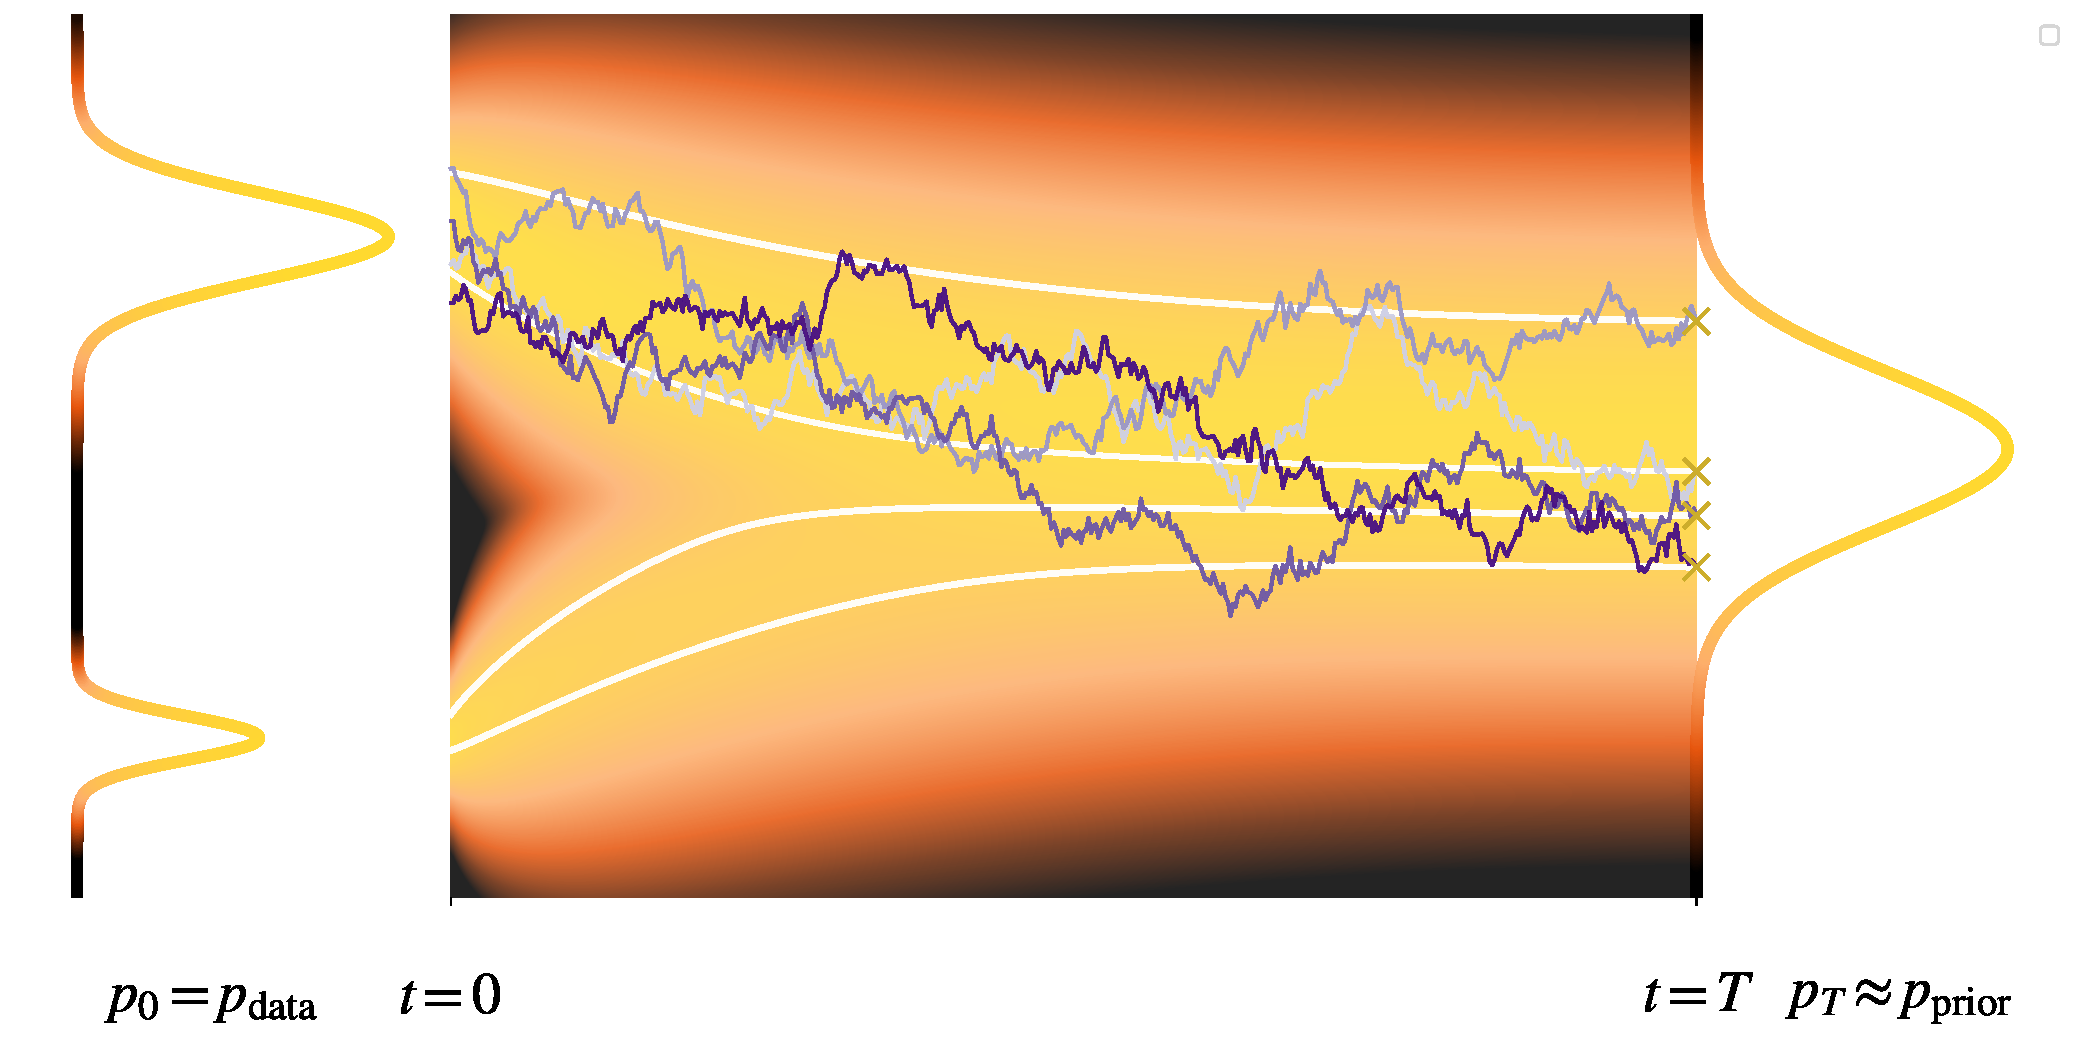
\includegraphics[width=\textwidth]{Images/PartB/reverse_sde_and_ode_trajectories.pdf}
    \caption{\textbfs{数据生成的逆时随机过程的可视化。} 
它从简单先验分布中抽取的样本开始 
（$p_{\mathrm{prior}}$）在$t=T$（表示为“$\times$”），向后进化 
及时使用反向SDE。产生的轨迹终止于 $t=0$ 
并共同形成目标双峰数据分布 
（$p_0 = p_{\mathrm{data}}$）。背景热图说明了如何 
概率密度逐渐从简单的高斯分布转变为 
复杂的目标分布。
\figcredit{由作者创建。}}
    \label{fig:sde-density-back-traj}
\end{figure}
直观上，从噪声生成数据可以通过“反转”前向过程来实现：从先验分布中采样的随机点开始，并及时向后演化以获得生成的样本。对于确定性系统（即 ODE），这个想法自然有效。由于不涉及随机性，反转时间只是意味着沿着与正向过程相同的路径追踪相反方向上的点的轨迹\footnote{从技术上讲，这对应于使用时间翻转替换$t \leftrightarrow T - t$.}来求解ODE。相比之下，SDE 在每个时间步都包含随机性，这意味着单个点可以沿着许多看似合理的随机轨迹演化。因此，逆向此类过程更加微妙\footnote{单纯地翻转时间并不能产生正确的逆向过程。}。虽然单个随机轨迹是不可逆的，但值得注意的是这些轨迹的分布是可以逆转的。这是由 \citet{anderson1982reverse} 的基本结果形式化的，它表明时间反转过程 $\{ \bar{\rvx}(t) \}_{t \in [0, T]}$\footnote{ 我们使用“bar”符号来区分反向过程 $\{ \bar{\rvx}(t) \}_{t \in [0, T]}$ 和正向过程 $\{ \rvx(t) \}_{t \in [0, T]}$，由正向过程的正向时间 SDE 定义。} 的正向过程\Cref{eq:sde_forward} 本身由定义明确的 SDE 管理。该逆时过程从 $T$ 演变为 $0$，其动态由下式给出：
\begin{mdframed}
\begin{align}\label{eq:sde_backward}
\begin{aligned}[t]
    \diff\bar{\rvx}(t) = \left[\mathbf{f}(\bar{\rvx}(t), t) {\color{orange} - g^2(t) \nabla_{\rvx} \log p_t(\bar{\rvx}(t))} \right] \diff t + g(t) \diff \bar{\rvw}(t), \\
    \hfill\bar{\rvx}(T) \sim p_{\mathrm{prior}} \approx p_T.
\end{aligned}
\end{align}
\end{mdframed}
这里，$\bar{\rvw}(t)$表示逆时标准维纳过程，定义为$\bar{\rvw}(t) := \rvw(T - t) - \rvw(T)$。

\rmkb{
在本章中，$t$ 表示原始扩散时钟：
$t=0$ 对应于数据，$t=T$ 对应于噪声。
因此，\Cref{eq:sde_backward}中的逆时SDE被集成
从$t=T$下降到$t=0$，所以$\diff t<0$沿着相反的过程。
同样地，可以引入一个正向运行的反向时钟
$s:=T-t$;除非另有说明，我们保留原始时钟$t$。
}

为了建立 \Cref{eq:sde_backward} 的直觉，我们在 \Cref{subsec:example-gaussian} 中提供了一个具有高斯数据分布和线性高斯动力学的具体示例。这一设置在分析上是易于处理的：可以直接使用基本微积分和线性代数推导时间反转公式，而无需调用 \citet{anderson1982reverse} 的完整一般理论。


请注意，随机性 ($g\neq 0$) 的存在引入了一个额外的校正项 $ -g^2(t) \nabla_{\rvx} \log p_t(\bar{\rvx}(t))$，它解释了扩散的影响，并确保反向动力学正确地再现由前向 SDE 引起的边缘分布的演化（请参阅 \Cref{subsec:fpe-sde-ode}）。

\paragraph{ 从概念上讲，为什么逆过程有效？} \Cref{subsec:reverse-sde-reason} 通过将反向时间 SDE 连接到 DDPM 变分框架（可选但富有洞察力），呈现了反向时间 SDE 的直观推导。在这里，我们提供了关于逆时动力学如何从噪声中恢复结构化数据的补充直觉。


乍一看，逆时间过程中布朗噪声的存在似乎是自相矛盾的。如果前向扩散将数据传播到噪声越来越大的配置中，则尚不清楚如何反转这一过程，特别是通过 $\bar{\rvw}(t)$ 引入额外随机性的过程，可以产生集中在数据流形附近的干净的结构化样本。关键在于反向时间 SDE 并没有注入任意随机性。扩散项 $g(t)\diff\bar{\rvw}(t)$ 始终与分数驱动的漂移 $- g^2(t)\nabla_{\rvx}\log p_t(\bar{\rvx}(t))$ 耦合。总之，这些术语相互平衡：分数引导轨迹走向更高密度的区域，而噪声则引入受控随机性，允许探索而不会压倒动态。

为了更清楚地看到这一点，请回到朗之万直觉 \Cref{eq:continuous-langevin}。当 $f(t)\equiv 0$, \Cref{eq:sde_backward} 读取
\[
\diff\bar{\rvx}(t)
= - g^2(t) \nabla_{\rvx}\log p_t\!\big(\bar{\rvx}(t)\big) \diff t
+ g(t)  \diff\bar{\rvw}(t).
\]
通过重新参数化时间向前 $s:=T-t$ （所以 $\diff t=-\diff s$)，并将布朗运动定律重命名为 $\diff\bar{\rvw}(t)=-\diff\rvw_s$。写作 $\bar{\rvx}_s:=\bar{\rvx}(T-s)$ 和 $\pi_s:=p_{T-s}$ 然后给出
\begin{align*}
    \diff\bar{\rvx}_s
&= g^2(T-s) \nabla\log \pi_s \big(\bar{\rvx}_s\big) \diff s
+ g(T-s) \diff\rvw_s
\\&=
2\tau(s) \nabla\log \pi_s\!\big(\bar{\rvx}_s\big) \diff s
+ \sqrt{2\tau(s)} \diff\rvw_s,
\quad
\tau(s):=\tfrac{1}{2}g^2(T-s).
\end{align*}
具有随时间变化的温度的 Langevin 形式 $\tau(s)$，针对不断发展的密度 $\pi_s$。根据特威迪公式 (\Cref{eq:tweedie})，分数方向 $\nabla\log \pi_s$ 指向每个时间片的条件干净信号，因此漂移不断“拉回”去噪结构。至关重要的是， $g(t)$ 是 \emph{退火} 沿着相反的轨迹。早期（$s\approx 0$, i.e., $t\approx T$), $g(T-s)$ 通常较大，因此注入的噪声更强，并且过程探索更广泛。作为 $s$ 增加， $g(T-s)$ 减少，随机项减弱，分数项占主导地位，将样本拉入高密度区域 $\pi_s$;通过 $s=T$ (i.e., $t=0$)，轨迹集中在数据流形附近。





\paragraph{反向时间 SDE 功能概述。}


与时间相关的分数如何发挥作用是令人着迷的
\[
\rvs(\rvx, t) := \nabla_{\rvx} \log p_t(\rvx)
\]
自然出现在 \Cref{eq:sde_backward}。一旦前向系数 $f(t)$ 和 $g(t)$ 已指定，分数是反向动态中唯一剩余的未知数。这就凸显了它的核心作用：有了分数在手，逆向过程就确定了，采样就相当于数值积分 \Cref{eq:sde_backward} 带有学习的分数。由于预言机分数通常缺乏封闭式表达，我们采用以下方法 \Cref{ch:score-based} 并训练神经网络 $\mathbf{s}_{\bm{\phi}}(\rvx, t)$ 通过分数匹配来近似；看到 \Cref{subsec:sde-train} 了解详情。替代 $\rvs(\rvx, t)$ 与 $\mathbf{s}_{\bm{\phi}}(\rvx, t)$ 在 \Cref{eq:sde_backward} 则完全指定反向动态。生成对应于求解反向时间 SDE $t = T$，从 $\rvx_T \sim p_{\mathrm{prior}}$, 至 $t = 0$。重要的是， \citet{anderson1982reverse} 证明正向和反向过程的边缘密度一致，确保样本在 $t=0$ 大约遵循 $p_{\mathrm{data}}$ 当 $p_{\mathrm{prior}} \approx p_T$。我们将进一步探讨这一点 \Cref{subsec:sde-sample}.






\subsection{生成的确定性过程（概率流 ODE）}\label{subsec:pf-ode}
 虽然 SDE 在 \Cref{eq:sde_backward} 引入随机性并可能增加生成样本的多样性，出现一个问题：
\begin{question}
    是否有必要使用SDE进行采样 \Cref{eq:sde_backward}?
\end{question}受 \citet{maoutsa2020interacting} 的启发，\citet{song2020score} 还引入了一种确定性过程，即 ODE，它演化出与前向 SDE 具有相同边缘分布的样本。这个过程$\{\tilde\rvx(t)\}_{t\in[0,T]}$\footnote{我们使用波形符来区分与正向和反向时间SDE相关的过程。展望未来，为了简单起见，我们省略了这种符号区别。}，称为 \emph{ 概率流 ODE (PF-ODE)}，由下式给出：
\begin{mdframed}
    \begin{equation}\label{eq:prob_ode_gt}
    \frac{\diff}{\diff t}\tilde\rvx(t) = \mathbf{f}(\tilde\rvx(t), t) - \frac{1}{2} g^2(t) \nabla_{\rvx} \log p_t(\tilde\rvx(t)).
    \end{equation}
\end{mdframed}

与 SDE 情况类似，可以用学习的近似值替换真实分数，并对从 $t = T$ 到 $t = 0$ 的逆时 ODE 进行积分以生成样本。具体来说，生成的样本（PF-ODE 在时间 $t=0$ 的解）采用以下形式
\[
\tilde\rvx(T) + \int_{T}^{0} \Big[ \mathbf{f}(\tilde\rvx(\tau), \tau) - \frac{1}{2} g^2(\tau)  \nabla_{\rvx} \log p_\tau(\tilde\rvx(\tau)) \Big]   \diff \tau,
\]
其中初始条件为 $\tilde\rvx(T) \sim p_{\mathrm{prior}}$。由于该积分在封闭形式下很难处理，因此实际生成依赖于数值求解器（例如，欧拉方法，请参阅 \Cref{eq:euler-maruyama}）。

与反向时间 SDE 相比，PF-ODE 具有两个关键优势：
\begin{itemize}
    \item ODE 可以在从 $t=0$ 到 $t=T$ 或从 $t=T$ 到 $t=0$ 的任一方向上积分，使用相同的方程公式，前提是在所选端点指定相应的初始条件。这种双向性与 SDE 形成鲜明对比，SDE 通常只允许前向时间积分。
    \item 它受益于为 ODE 开发的各种成熟、现成的数值求解器。
\end{itemize}


我们强调，PF-ODE并不是通过简单地去掉\Cref{eq:sde_backward}中的扩散项得到的；值得注意的是，$\frac{1}{2}$ 的漂移项中的因子有一个原则性的起源。在高层次上，\Cref{eq:prob_ode_gt} 通过选择 ODE 的漂移而产生，使其演化保留与 \Cref{eq:sde_forward} 中的前向 SDE 相同的边缘密度。确保边缘对齐的基本原理（即福克尔-普朗克方程~\citep{oksendal2003stochastic}）将在下一节中详细介绍。


\clearpage
\newpage



\section{前向与反向 SDE 及 PF-ODE 的边缘分布一致性}\label{subsec:fpe-sde-ode}
\begin{figure}[th!]

    \centering
    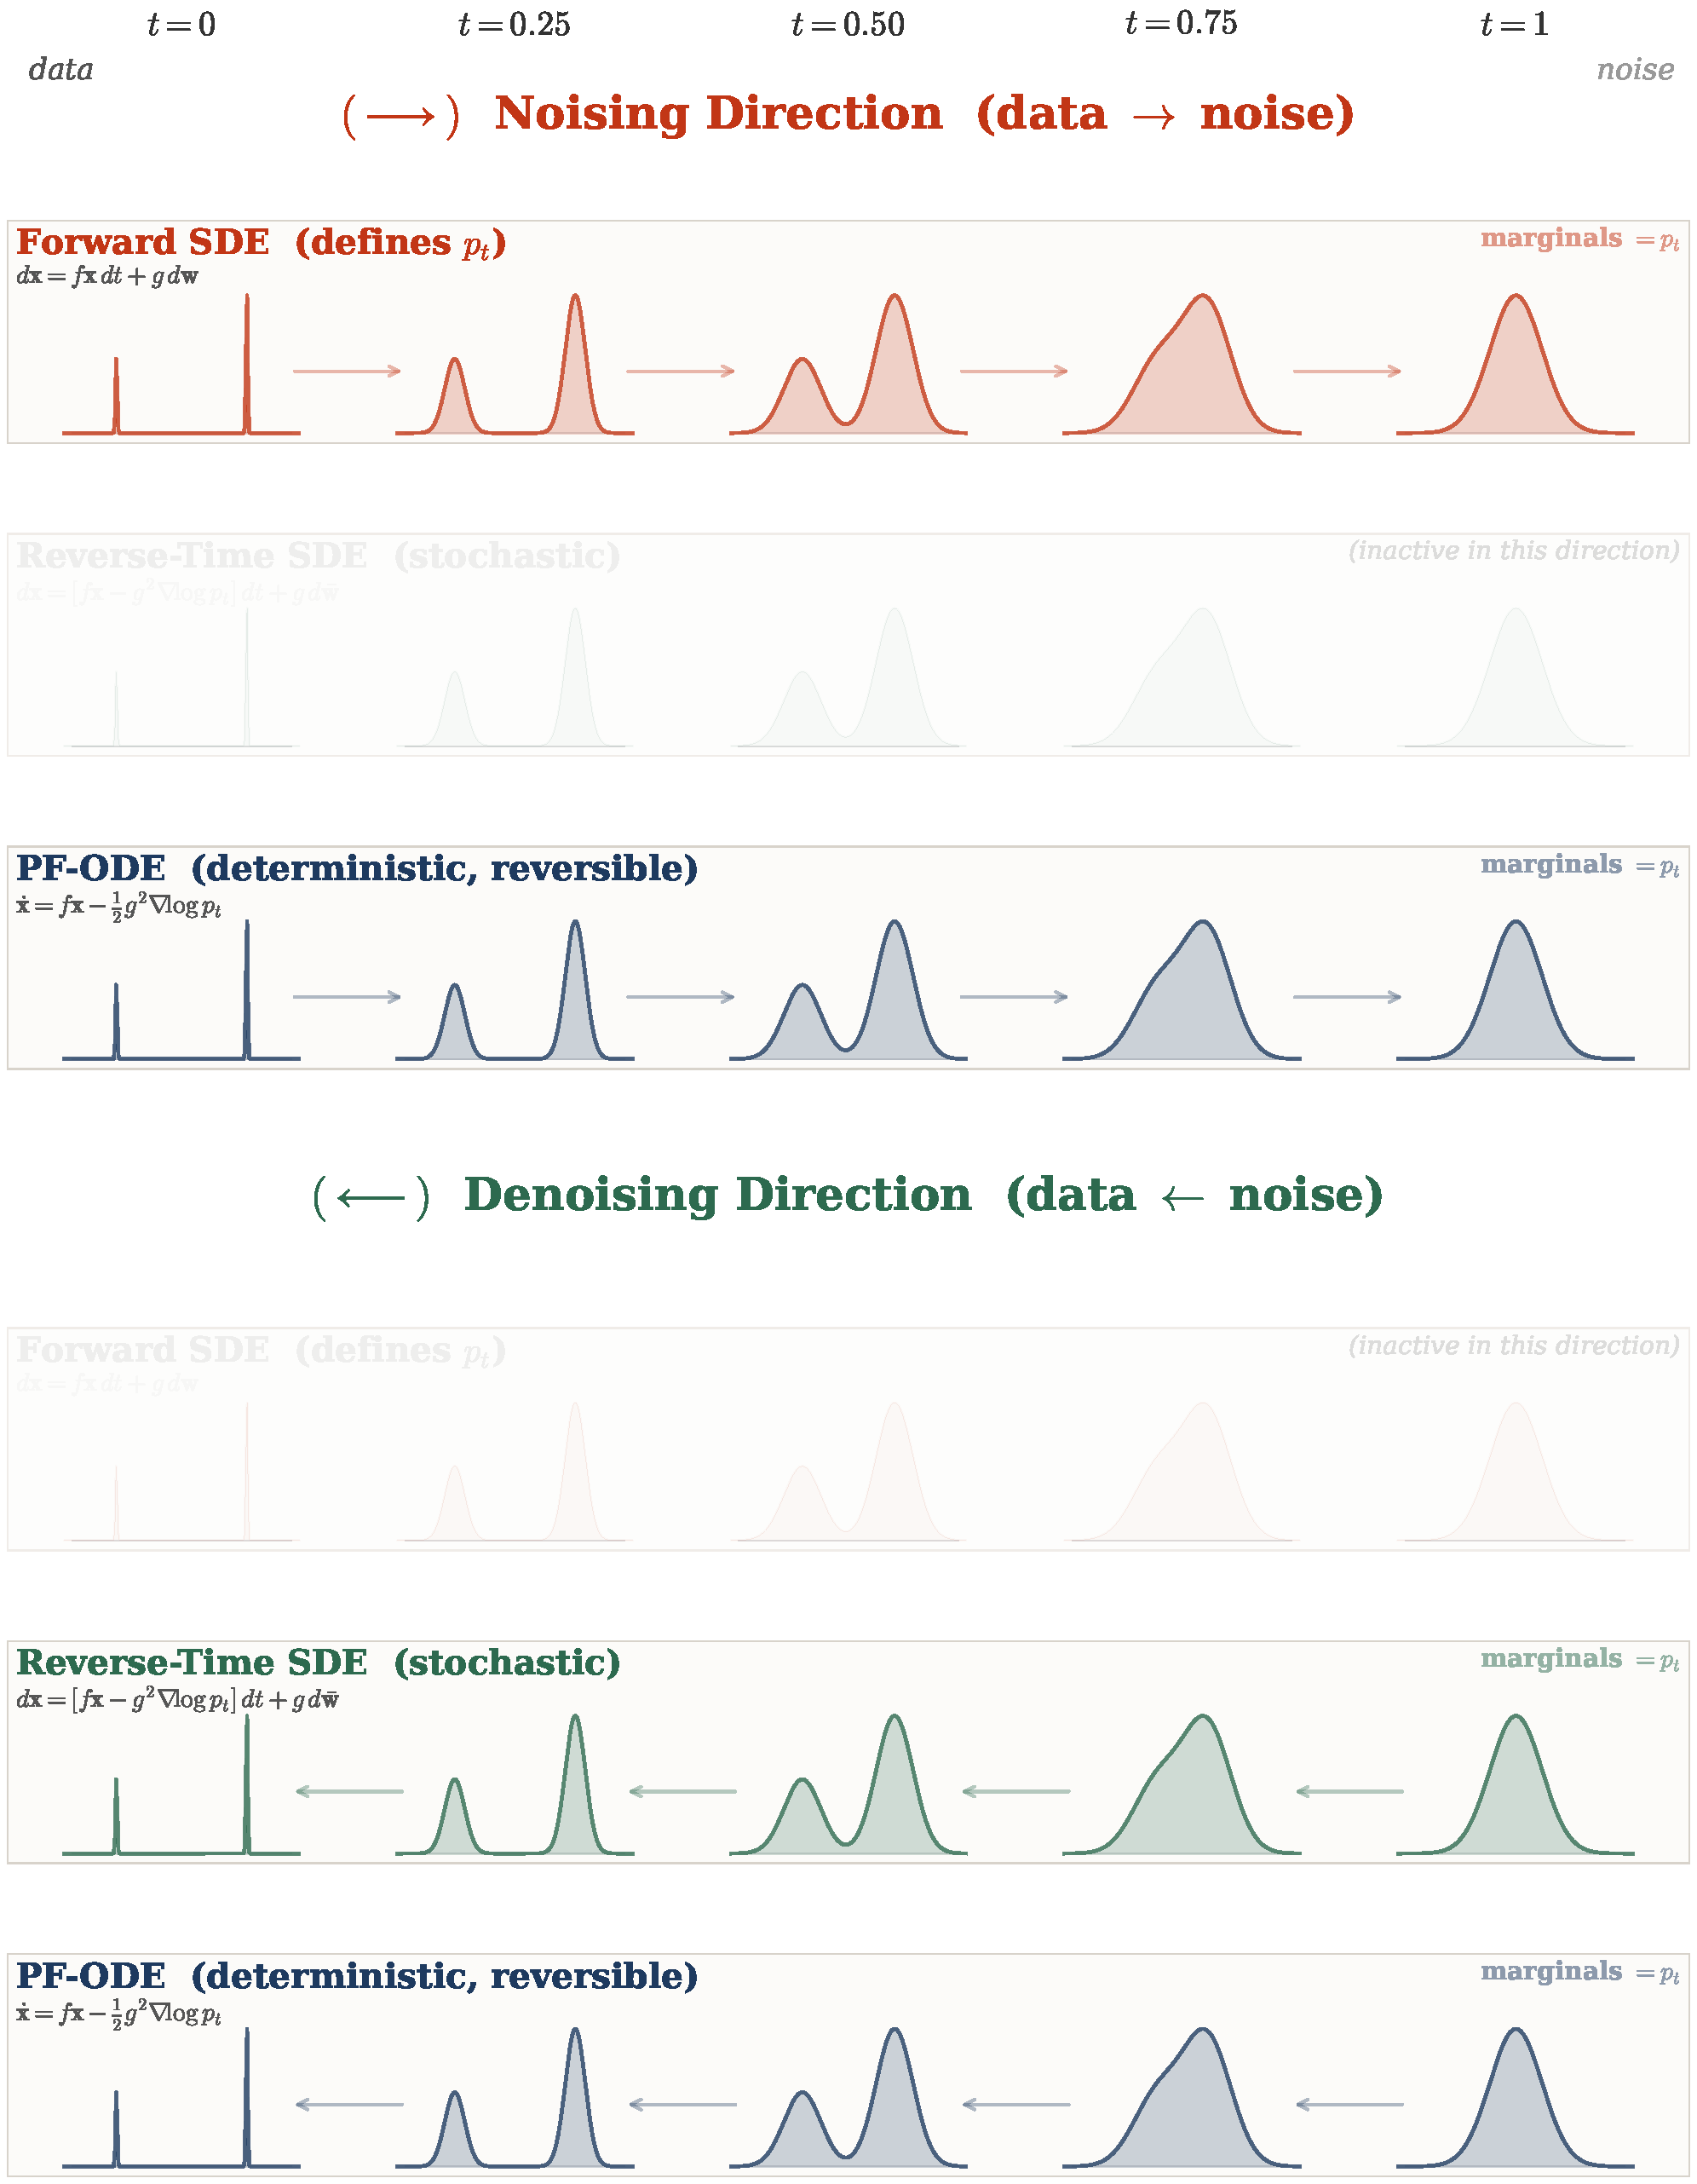
\includegraphics[width=\linewidth]{Images/PartB/score_sde_three_dynamics.pdf}
\caption{\textbfs{三种动态共享相同的边缘 $p_t$.}
\textbfs{上面板：噪声方向。}
前向 SDE，用作锚参考，定义边缘
$p_t$ 通过将数据扩散到高斯先验。当 PF-ODE 确定性地遵循相同的边缘路径时 \emph{及时向前运行}. \textbfs{下面板：去噪方向。}
反向时间 SDE 和 PF-ODE \emph{时间向后运行} 按照福克尔-普朗克方程的保证，反向产生相同的边缘。反向时间 SDE 提供随机去噪过程，而 PF-ODE 提供确定性去噪过程。因此，重复的密度快照是有意为之的：这些过程在一次性边缘水平上一致，但在样本水平动态方面有所不同。 PF-ODE 出现在两个面板中，因为它是可以在任一时间方向上积分的确定性流。
\figcredit{由作者使用人工智能辅助编码创建。}}
    \label{fig:score-sde-three-dynamics}
    \vspace{-2cm}
\end{figure}
在本节中，我们介绍 \emph{福克尔-普朗克方程} 作为控制扩散模型的中心原则。它描述了概率密度在噪声动态下如何演变，并作为存在随机性时变量变换公式的自然模拟（参见 \Cref{app:continuity}）。从定义边缘的前向扩散过程开始 $p_t$我们解释了反向时间 SDE 和 PF-ODE 是如何设计来重现相同的边缘族的。然后，我们通过高斯示例具体化这一原理，其中可以直接、显式地计算反向时间 SDE 和 PF-ODE。











\subsection{福克尔-普朗克方程确保边缘密度对齐}
扩散模型的一个中心概念是 \emph{不同的过程可以导致相同的边缘分布序列} （我们将在本小节稍后进行说明）。目标是构建一个能够转变的流程 $p_{\mathrm{prior}}$ 进入 $p_{\mathrm{data}}$ 通过跨时间调整边缘，特别是在 $t=0$。该过程的具体形式是次要的，只要它易于处理并允许有效采样。这自然会引出一个基本问题：


\begin{question}
我们如何确保不同的过程产生相同的边缘分布？
\end{question}

回到我们的设置，一旦指定了前向 SDE，它就定义了从 $p_{\mathrm{data}}$ 到 $p_{\mathrm{prior}}$ 的边缘密度的演变。然后构造反向时间 SDE 和 PF-ODE，以便它们的轨迹产生与正向过程的轨迹完全匹配的边缘分布。这种对应关系的关键在于福克尔-普朗克方程，该方程控制着扩散过程中边缘密度如何演变。 \Cref{fig:score-sde-three-dynamics} 中提供了说明。以下定理~\citep{anderson1982reverse,song2020score} 为这种连接奠定了基础：
\thmp{通过福克尔-普朗克方程进行边缘对齐}{fpe}{
考虑前向 SDE
\[
\diff \rvx(t)
=
\rvf(\rvx(t),t)\diff t
+
g(t)\diff \rvw(t),
\qquad
\rvx(0)\sim p_0=p_{\mathrm{data}}.
\]
在标准正则条件下，其边缘密度 $p_t$ 演化
根据福克尔-普朗克方程
\begin{align}\label{eq:fp_general}
\begin{aligned}
\partial_t p_t(\rvx)
&=
-\nabla_{\rvx}\cdot
\bigl[\rvf(\rvx,t)p_t(\rvx)\bigr]
+
\tfrac12 g^2(t)\Delta_{\rvx}p_t(\rvx)
\\
&=
-\nabla_{\rvx}\cdot
\bigl[\rvv(\rvx,t)p_t(\rvx)\bigr],
\end{aligned}
\end{align}
其中 $\Delta_{\rvx}$ 表示拉普拉斯算子，
\[
\rvv(\rvx,t)
:=
\rvf(\rvx,t)
-
\tfrac12 g^2(t)
\nabla_{\rvx}\log p_t(\rvx).
\]

重要的是，同一个边缘分布族
$\{p_t\}_{t\in[0,T]}$可以通过两种不同的动力来实现：

\begin{enumerate}
\item[\textup{(i)}]
\emph{PF-ODE}
\[
\frac{\diff\tilde\rvx(t)}{\diff t}
=
\rvv(\tilde\rvx(t),t).
\]
从 $\tilde\rvx(0)\sim p_0$ 开始，从 $0$ 向前求解到 $T$
给出 $\tilde\rvx(t)\sim p_t$。
等价地，从$\tilde\rvx(T)\sim p_T$开始并求解相同的ODE
从 $T$ 向后到 $0$ 遵循相同的反向边缘。

\item[\textup{(ii)}]
\emph{反时限SDE}
\[
\diff\bar\rvx(t)
=
\Bigl[
\rvf(\bar\rvx(t),t)
-
g^2(t)\nabla_{\rvx}\log p_t(\bar\rvx(t))
\Bigr]\diff t
+
g(t)\diff\bar\rvw(t).
\]
从$\bar\rvx(T)\sim p_T$开始，这个SDE在时间上向后求解
$t=T$ 至 $t=0$。沿着这个反向演化，它的边缘分布在
时间 $t$ 是
\[
\bar\rvx(t)\sim p_t.
\]
\end{enumerate}

因此，反向时间 SDE 和 PF-ODE 可以具有相同的边缘分布
在每个噪声水平，即使一个是随机的，另一个是
确定性的。
}{
\Cref{app-sec:scoresde-fpe-proof} 中提供了证明，而 \Cref{subsec:fpe-reason} 使用概率边缘化技术提供了福克尔-普朗克方程背后的进一步直觉。
}

\paragraph{固定边缘的多个条件分布。}
了解 PF-ODE 如何传输 $p_{\mathrm{data}}$ 及时向前（或等效 $p_{\mathrm{prior}}$ 相反），考虑 \emph{流映射} $\bPsi_{s \to t}: \mathbb{R}^D \to \mathbb{R}^D$，其中 $\bPsi_{s \to t}(\rvx_s)$ 表示此时的PF-ODE解 $t$ 初始化自 $\rvx_s$ 当时 $s$，任何时间 $s, t \in[0,T]$。换句话说，这张映射有一个初始状态 $\rvx_s$ 并直接跳转到其状态 $t$:
\begin{align}\label{eq:flow-map-def}
\bPsi_{s \to t}(\rvx_s) \coloneqq \rvx_s + \int_s^t \rvv(\rvx_\tau, \tau)\mathrm{d}\tau,
\end{align}
有速度场
\begin{align*}
\rvv(\rvx, \tau) := \rvf(\rvx, \tau) - \frac{1}{2} g^2(\tau)\nabla_{\rvx}\log p_\tau(\rvx).
\end{align*}
此处，积分捕获沿 PF-ODE 轨迹累积的净位移。术语 \emph{流映射} 在微分方程、动力系统和连续介质力学中确实是经典：它表示从其时间位置携带状态的映射 $s$ 到达当时的位置 $t$ 在给定的动态下。速度场
$\rvv(\rvx,t)$ 描述瞬时运动，而流图
$\bPsi_{s\to t}$ 记录有限时间间隔内的累积运动~\citep{arnold1988geometrical,chorin1993mathematical}\footnote{这张映射背后的物理思想要古老得多。十八世纪的流体力学已经通过速度场和跟踪材料粒子的演化来研究运动，特别是在欧拉和拉格朗日的基础著作中
~\citep{euler1757fluid,lagrange1783fluid}.}。我们在整本书中都以这种标准的数学和物理意义使用该术语，特别是在讨论快速扩散生成器时 \Cref{ch:distillation,ch:fast-scratch}。在温和平滑度假设下 $\rvv$，流映射
$\bPsi_{s \to t}: \mathbb{R}^D \to \mathbb{R}^D$ 是平滑双射\footnote{
剧透：PF-ODE 流映射 $\bPsi_{s\to t}$ 正是承载的归一化流（NF）双射 $p_s$ 至 $p_t$ （详见
\Cref{sec:flow-based-method}）。不同之处在于，一旦前向 SDE 及其边缘密度固定，PF-ODE 公式就唯一指定其相关的速度场， $\rvv(\rvx,t)
=
\rvf(\rvx,t)
-\frac{1}{2}g^2(t)\nabla_{\rvx}\log p_t(\rvx)$，而归一化流或连续时间归一化流直接参数化并学习速度场。两者都依赖于相同的变量连续变化原理。
}。对于任何 $t\in[0,T]$， \emph{前推密度} 定义为
\[
p_t^{\mathrm{fwd}}(\rvx_t) := \int \delta\bigl(\rvx_t - \bPsi_{0 \to t}(\rvx_0)\bigr)\, p_{\mathrm{data}}(\rvx_0) \,\diff \rvx_0,
\]
表示 $\bm{\Psi}_{0\to t} \sharp p_{\mathrm{data}}$，代表时间上的分布 $t$ 下 $\bm{\Psi}_{0\to t}$。定理~\ref{thm:fpe} 确保 $p_t^{\mathrm{fwd}} = p_t$，其中 $p_t$ 是前向 SDE 的边缘密度，相当于确定性 PF-ODE 和随机核：
\[
p_t(\rvx_t) = \int p_t(\rvx_t |\rvx_0)\, p_{\mathrm{data}}(\rvx_0)\,\diff \rvx_0
= \int \delta\bigl(\rvx_t - \bm{\Psi}_{0\to t}(\rvx_0)\bigr)\, p_{\mathrm{data}}(\rvx_0)\,\diff \rvx_0.
\]

这意味着无限多个条件 $Q_t(\rvx_t |\rvx_0)$ 产量相同 $p_t(\rvx_t)$，例如：
\begin{itemize}
  \item \textbfs{随机（无模拟）：} $Q_t(\rvx_t |\rvx_0) = p_t(\rvx_t |\rvx_0)$,
  \item \textbfs{确定性（需要 ODE 求解）：} $Q_t(\rvx_t |\rvx_0) = \delta\bigl(\rvx_t - \bm{\Psi}_{0\to t}(\rvx_0)\bigr)$,
  \item \textbfs{混合物：} $Q_t(\rvx_t |\rvx_0) = \lambda p_t(\rvx_t |\rvx_0) + (1-\lambda)\delta\bigl(\rvx_t - \bm{\Psi}_{0\to t}(\rvx_0)\bigr)$, $\lambda\in[0,1]$.
\end{itemize}
这种非唯一性 $Q_t(\rvx_t |\rvx_0)$ 源于边缘约束不能唯一确定条件分布的事实。这个概念再次出现在 \Cref{subsec:fm-framework} 和 \Cref{subsec:ddim}。特别是，存在一整套反向时间 SDE，它们与相同的边缘条件一致。 $p_t$.

\msg{观察}{Matching Prescribed Marginal Densities}{
多个过程可以产生相同的边缘密度序列；真正重要的是满足福克尔-普朗克方程。这一基本见解为我们设计生成过程提供了非凡的灵活性，这些过程从 $ p_{\mathrm{prior}} $ 至 $ p_{\mathrm{data}} $，反之亦然。
}
福克尔-普朗克方程是扩散模型的核心，植根于基本原理 \emph{变量变换公式} 概率密度（参见 \Cref{app:continuity} 用于系统治疗）。这一原则远非一个次要的技术细节，而是在我们的整个开发过程中反复出现，尤其是在 \Cref{sec:flow-matching-framework}.





\subsection{可计算示例：高斯动力学的演化}\label{subsec:example-gaussian}
当 $p_{\mathrm{data}}$ 是正态分布（或高斯混合），分数函数接受封闭式表达式。这使得它成为建立关于扩散过程的直觉的理想设置：我们可以仅使用基本微积分来显式导出反向时间 SDE 和 PF-ODE，而无需借助高级数学工具。在本小节中，我们将说明这些方程在这种易于处理的情况下的表现。



\paragraph{使用高斯函数精确计算反向时间 SDE。}
 当 $p_{\mathrm{data}}$ 为高斯分布，公式为 \Cref{eq:sde_backward} 可以直接推导，无需依赖一般理论和证明 \citet{anderson1982reverse}。为了说明核心思想，我们考虑一维情况；以同样的方式扩展到更高的维度。从正向SDE开始
\[
\diff x(t)  =  f(t)  x(t)  \diff t  +  g(t)  \diff w_t,
\]
并采取一小段欧拉步长 $\Delta t>0$:
\[
x_{t+\Delta t}  =  a  x_t  +  r  \epsilon,
\]
其中 $a:=1+f(t)\Delta t$, $r:=g(t)\sqrt{\Delta t}$, 和 $ \epsilon\sim\mathcal N(0,1)$。等价地，前向一步转移核是高斯的：
\[
x_{t+\Delta t}   |   x_t  \sim  \mathcal N\!\big(\cdot;a  x_t,   r^2\big).
\]
自 $p_{\mathrm{data}}$ 假设为高斯分布，当前时刻的边缘 $t$ 也是高斯分布，其形式如下：
\[
x_t \sim \mathcal N(\cdot;m_t,   s_t^2),
\]
对于某些标量 $m_t$ 和 $s_t$。因此，调节相当于将两个高斯相乘并重新归一化。这使得代数保持基本。

根据贝叶斯规则，条件密度在常数范围内是先验核和转换核的乘积：
\begin{align*}
    p(x_t   |   x_{t+\Delta t})  &\propto p(x_{t+\Delta t} | x_t   ) p_t(\rvx_t) \\&\propto
\exp\Big(-\frac{(x_t-m_t)^2}{2s_t^2}\Big)  
\exp\Big(-\frac{(x_{t+\Delta t}-a  x_t)^2}{2r^2}\Big).
\end{align*}
指数是二次 $x_t$。展开平方和分组项可以准确显示哪些系数重要：
\[
-2\log p(x_t   |   x_{t+\Delta t})
 = 
A  x_t^2  -  2 B  x_t  +  \text{const},
\]
与
\[
A:=\frac{1}{s_t^2}+\frac{a^2}{r^2},\quad
B:=\frac{m_t}{s_t^2}+\frac{a  x_{t+\Delta t}}{r^2}.
\]
这里 $A$ 是精度之和（先验精度加上通过传输的转换内核精度 $a$），同时 $B$ 是对应的目标的精确加权总和。有了这些，完成平方就可以在一行中得到后验：
\[
A x_t^2 - 2 B x_t
  =  
A\Big(x_t-\frac{B}{A}\Big)^2  -  \frac{B^2}{A},
\]
所以条件分布是带方差的高斯分布 $1/A$ 和的意思 $B/A$:
\[
\Var(x_t   |   x_{t+\Delta t})   =   \frac{1}{\frac{1}{s_t^2}+\frac{a^2}{r^2}},
\qquad
\mathbb E[x_t   |   x_{t+\Delta t}]   =  
\frac{\frac{m_t}{s_t^2}+\frac{a  x_{t+\Delta t}}{r^2}}{\frac{1}{s_t^2}+\frac{a^2}{r^2}}.
\]
这些封闭形式已经描述了任何小 $\Delta t$。为了读取反向时间 SDE，我们现在将它们扩展为小的 $\Delta t$。使用 $a=1+f(t)\Delta t$ 和 $r^2=g^2(t)\Delta t$。作为 $\Delta t\to 0$，贡献 $\frac{a^2}{r^2}\sim \frac{1}{g^2(t)\Delta t}$ 主导精度，因此方差变为
\[
\Var(x_t   |   x_{t+\Delta t})
= \left(\frac{1}{s_t^2}+\frac{a^2}{r^2}\right)^{-1}
= g^2(t)  \Delta t  +  \mathcal{O}(\Delta t^2),
\]
这告诉我们反向步骤具有相同的扩散尺度 $g(t)$ 作为前进的一步。对于平均值，扩大比率 $B/A$ 到第一笔订单：
\[
\mathbb E[x_t   |   x_{t+\Delta t}]
  =  x_{t+\Delta t}
 +  \Delta t\left[
-\left(f(t)+\frac{g^2(t)}{s_t^2}\right)  x_{t+\Delta t}
 +  \frac{g^2(t)}{s_t^2}  m_t
\right]  +  \mathcal{O}(\Delta t^2).
\]

将均值和方差放在一起产生一步反向转移核
\[
x_t    |    x_{t+\Delta t}
 \sim 
\mathcal N\!\left(
x_{t+\Delta t} + \Delta t\!\left[-\left(f+\frac{g^2}{s_t^2}\right)  x_{t+\Delta t} + \frac{g^2}{s_t^2}  m_t\right],
 g^2  \Delta t\right)
 +  \mathcal{O}(\Delta t^2).
\]
这被认为是 Euler--Maruyama 更新，从
$t+\Delta t$ 至 $t$:
\[
x_t - x_{t+\Delta t}
= \Delta t\!\left[-\left(f+\frac{g^2}{s_t^2}\right) x_{t+\Delta t}
+ \frac{g^2}{s_t^2} m_t\right]
+ g\sqrt{\Delta t}\,\epsilon.
\]
这个向后漂移可以用分数来写，因为对于高斯边缘 $p_t=\mathcal N(m_t,s_t^2)$,
\[
\partial_x \log p_t(x) = -\frac{x-m_t}{s_t^2}
 \Longrightarrow
-\left(f+\frac{g^2}{s_t^2}\right)x
+\frac{g^2}{s_t^2}m_t
=
-\left[f x-g^2\partial_x\log p_t(x)\right].
\]
因此，让 $\Delta t\to0$ 给出原始扩散时钟上的逆时SDE，
\[
\diff \bar x(t)
=
\left[
f(t)\bar x(t)
-
g^2(t)\partial_x\log p_t(\bar x(t))
\right]\diff t
+
g(t)\diff\bar w(t),
\qquad t:T\to0.
\]
这与一般的逆时SDE完全匹配
\Cref{eq:sde_backward}。在向量形式中，标量导数
$\partial_x\log p_t$ 替换为
$\nabla_{\rvx}\log p_t$.

\paragraph{使用高斯函数精确计算 PF-ODE。}
当假设数据分布为高斯分布时，我们也可以直接推导PF-ODE公式，避免了福克尔-普朗克方程等繁琐的机械操作。最后，我们将看到 PF-ODE 的边缘密度与正向 SDE 和反向时间 SDE 的边缘密度一致，这为将要讨论的 Fokker-Planck 理论提供了建设性的验证。 \Cref{subsec:fpe-sde-ode}。假设 $x_t\sim\mathcal N(\cdot;m_t,s_t^2)$ 当时 $t$。尺寸的一个小的确定性步骤 $\Delta t$ 可以写成平滑图
\[
x_{t+\Delta t}=\Phi_{t,\Delta t}(x_t)
= x_t + \Delta t v_t(x_t) + \mathcal{O}(\Delta t^2),
\]
这只是一阶泰勒展开 $\Delta t$。我们的目标是构建一个速度场，其确定性流再现相同的高斯边缘演化。一个特别简单的选择是仿射速度场
\[
v_t(x)=a_t x+b_t.
\]
由于仿射动力学保持高斯性，我们可以确定 $a_t$ 和 $b_t$
通过将均值和方差的演化与前向 SDE 的演化相匹配。将其插回到步骤中给出
\[
x_{t+\Delta t}=(1+\alpha_t \Delta t) x_t+\beta_t \Delta t+\mathcal{O}(\Delta t^2),
\qquad
\alpha_t:=a_t,\ \ \beta_t:=b_t.
\]























现在我们将 $x_t\sim\mathcal N(\cdot;m_t,s_t^2)$ 推入该映射并跟踪一阶均值和方差：
\begin{align*}
\mathbb E[x_{t+\Delta t}]
&= m_t+\Delta t(\alpha_t m_t+\beta_t)+\mathcal{O}(\Delta t^2),
\\
\Var(x_{t+\Delta t})
&= s_t^2+\Delta t (2\alpha_t s_t^2)+\mathcal{O}(\Delta t^2).
\end{align*}
另一方面，正向 SDE $\diff x=f(t) x \diff t+g(t) \diff w_t$ 具有基本矩公式（参见 \Cref{eq:mean-var-evolution}）：
\[
m_t' = f(t) m_t,
\qquad
(s_t^2)' = 2 f(t) s_t^2 + g^2(t).
\]
匹配 $\Delta t$ 的系数得出
\[
\alpha_t = f(t)+\frac{g^2(t)}{2 s_t^2},
\qquad
\beta_t = - \frac{g^2(t)}{2 s_t^2} m_t.
\]

有了这些选择，步骤就变成了
\[
x_{t+\Delta t}
= x_t + \Delta t\!\left[\Big(f(t)+\frac{g^2(t)}{2s_t^2}\Big)x_t
-\frac{g^2(t)}{2s_t^2} m_t\right]+\mathcal{O}(\Delta t^2).
\]
由于对于高斯 $p_t=\mathcal N(m_t,s_t^2)$ 我们有 $\partial_x\log p_t(x)=-(x-m_t)/s_t^2$，因此我们可以将括号重写为
$f(t) x_t - \tfrac12 g^2(t) \partial_x\log p_t(x_t)$。
因此，
\[
x_{t+\Delta t}
= x_t + \Delta t\Big[f(t) x_t - \tfrac12 g^2(t) \partial_x\log p_t(x_t)\Big] + \mathcal{O}(\Delta t^2).
\]
最后，除以 $\Delta t$ 并令 $\Delta t\to 0$ 得出 PF-ODE
\[
x'(t)  =  f(t) x(t)  -  \tfrac12 g^2(t) \partial_x\log p_t\!\big(x(t)\big).
\]

要了解为什么此 ODE 与正向 SDE（和反向时间 SDE）具有相同的边缘，请观察上面的漂移是线性加上偏移的。因此，$x(t)$ 仿射地依赖于 $x(0)$，并且仿射映射将高斯函数发送到高斯函数。此外，沿该 ODE 的均值 $m_t$ 和方差 $s_t^2$ 满足与前向 SDE 完全相同的两个标量 ODE（通过我们的匹配），具有相同的初始值。因此，$p_t=\mathcal N(m_t,s_t^2)$ 对于每次 $t$ 的两种演化都是相同的。





\clearpage
\newpage




\section{分数 SDE 的训练与采样}\label{sec:scoresde-training-sampling}

\subsection{训练}\label{subsec:sde-train}
基于 \Cref{ch:score-based} 的理念，我们使用时间条件神经网络来近似预言机分数 $\nabla_{\rvx} \log p_t(\rvx)$ 
\[
\mathbf{s}_{\bm{\phi}} = \mathbf{s}_{\bm{\phi}}(\rvx, t)
\]
在所有 $t\in[0,T]$ 中，通过最小化 \Cref{eq:sm} 中的分数匹配目标：
\begin{equation*}
\mathcal{L}_{\text{SM}}(\bm{\phi}; \omega(\cdot)) := \frac{1}{2} \mathbb{E}_{t\sim p_{\text{time}}}  \mathbb{E}_{\rvx_t \sim p_t}\left[\omega(t) \left\|\mathbf{s}_{\bm{\phi}}(\rvx_t, t) - \nabla_{\rvx} \log p_t(\rvx_t)\right\|_2^2\right],
\end{equation*}
其中 $p_{\text{time}}$ 是某种时间分布（例如，$[0,T]$ 上的均匀分布），$\omega(\cdot)$ 是时间加权函数。

\begin{figure}[th!]
    \centering
    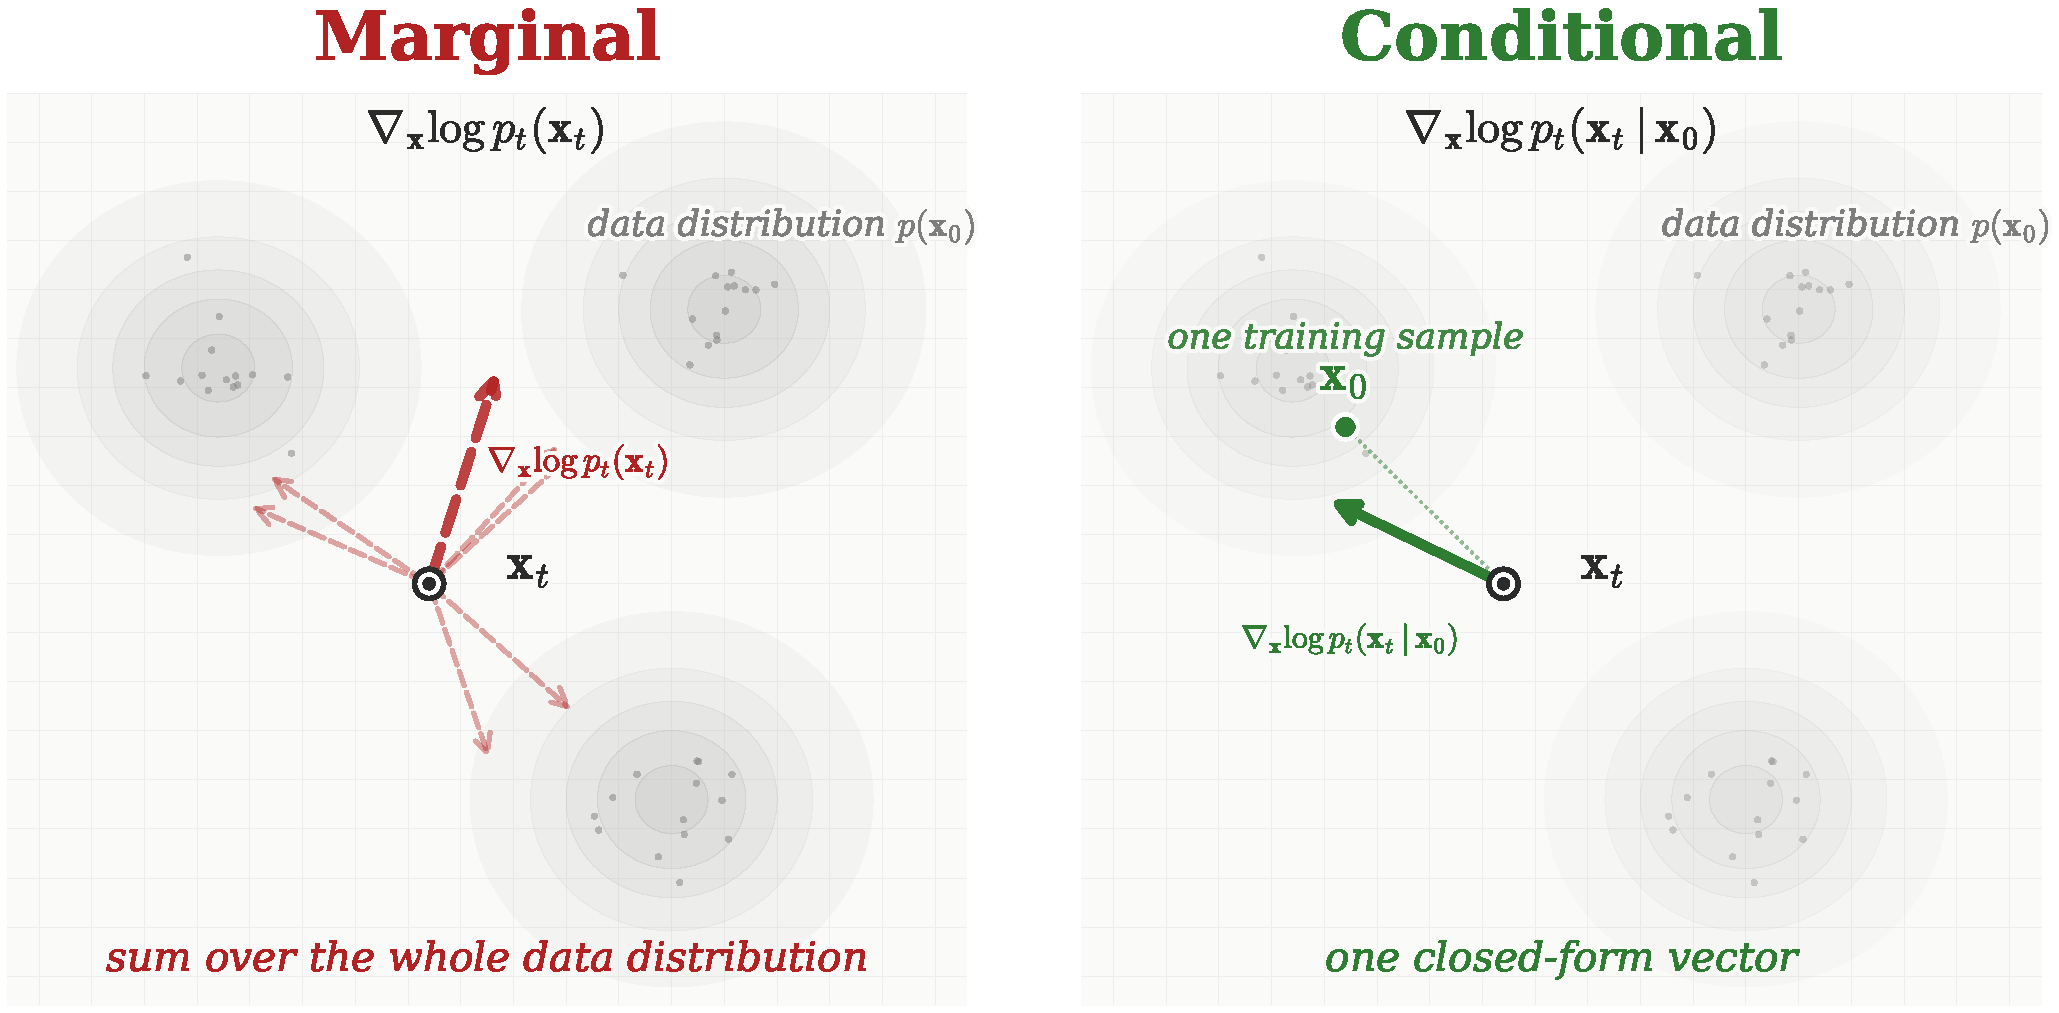
\includegraphics[width=\linewidth]{Images/PartB/denoising_score_matching.pdf}
    \caption{\textbfs{去噪分数匹配技巧。}
    \textbfs{(左)}
    对于固定噪声样本 $\rvx_t$，边缘分数
    $\nabla_{\rvx_t}\log p_t(\rvx_t)$ 指向嘈杂的区域
    样本的可能性更大。直接计算它需要结合
    来自所有可能的干净样本 $\rvx_0$ 的贡献
    生产了$\rvx_t$，一般很难处理。
    \textbfs{(右)}
    然而，在训练期间，干净的样本 $\rvx_0$ 用于生成
    $\rvx_t$ 是已知的。对于高斯扰动，相应的
    条件分数
    $\nabla_{\rvx_t}\log p_t(\rvx_t|\rvx_0)$ 为封闭形式，
    提供一个简单向量作为回归目标。跨训练
    例如，这些条件分数向量平均到边缘
    分数。因此，去噪分数匹配可以学习所需的边缘分数，而无需
直接回归通常难以处理的分数
$\nabla_{\rvx_t}\log p_t(\rvx_t)$，其评估需要求平均值
数据分布中所有可能的样本。
    \figcredit{由作者使用AI辅助编码创建。}}
    \label{fig:score-and-denoising-score}
\end{figure}

避免依赖棘手的预言机分数 $\nabla_{\rvx} \log p_t(\rvx)$，DSM 损失 \Cref{eq:dsm-loss} 已就业。以数据点为条件 $\rvx_0$，这种方法允许使用分析上易于处理的分数 $\nabla_{\rvx_t} \log p_t(\rvx_t|\rvx_0)$ 通过 \Cref{eq:score-gaussian-formula}，具体示例在 \Cref{sec:instances}。具体来说，我们利用以下损失函数：
\begin{mdframed}
    \begin{equation}\label{eq:conti-dsm_loss-real}
\begin{aligned}
     &\mathcal{L}_{\text{DSM}}(\bm{\phi}; \omega(\cdot)) := \\
     &\frac{1}{2} \mathbb{E}_{t}  \mathbb{E}_{\rvx_0} \mathbb{E}_{ p_t(\rvx_t|\rvx_0)} \Big[\omega(t)\norm{\mathbf{s}_{\bm{\phi}}(\rvx_t, t) - \nabla_{\rvx_t} \log p_t(\rvx_t|\rvx_0)}_2^2 \Big],
\end{aligned}
\end{equation}
\end{mdframed}
其中 $\rvx_0 \sim p_{\mathrm{data}}$. \Cref{eq:conti-dsm_loss-real} 可以解释为连续时间对应的 \Cref{eq:nscn}，用积分代替离散情况下的求和。与定理中的结果类似~\ref{thm:sm-dsm}，最小化 \Cref{eq:conti-dsm_loss-real} 唯一确定如下：

\proppp{DSM 的最小化}{dsm-minimizer}{
最小化器 $\mathbf{s}^*$ 满足
\begin{align}\label{eq:optimal-score}
\begin{aligned}
    \mathbf{s}^*(\rvx_t, t) 
    = \mathbb{E}_{\rvx_0 \sim p(\rvx_0 | \rvx_t)} \big[ \nabla_{\rvx_t} \log p_t(\rvx_t | \rvx_0) \big]= \nabla_{\rvx_t} \log p_t(\rvx_t),
\end{aligned}
\end{align}
对于几乎所有 $\rvx_t \sim p_t$ 和 $t \in [0,T]$. }{ 
DSM目标可以理解为最小二乘误差问题。具体来说，在每个时间 $t$，最优分数函数由对数条件密度梯度的条件期望给出，在贝叶斯规则下，其等价于对数边缘密度的梯度。详细证明见附录~\ref{app-sec:min-dsm}.
}


\subsection{采样和推理}\label{subsec:sde-sample}
\begin{figure}[th!]
    \centering
    \vspace{-0.8cm}
    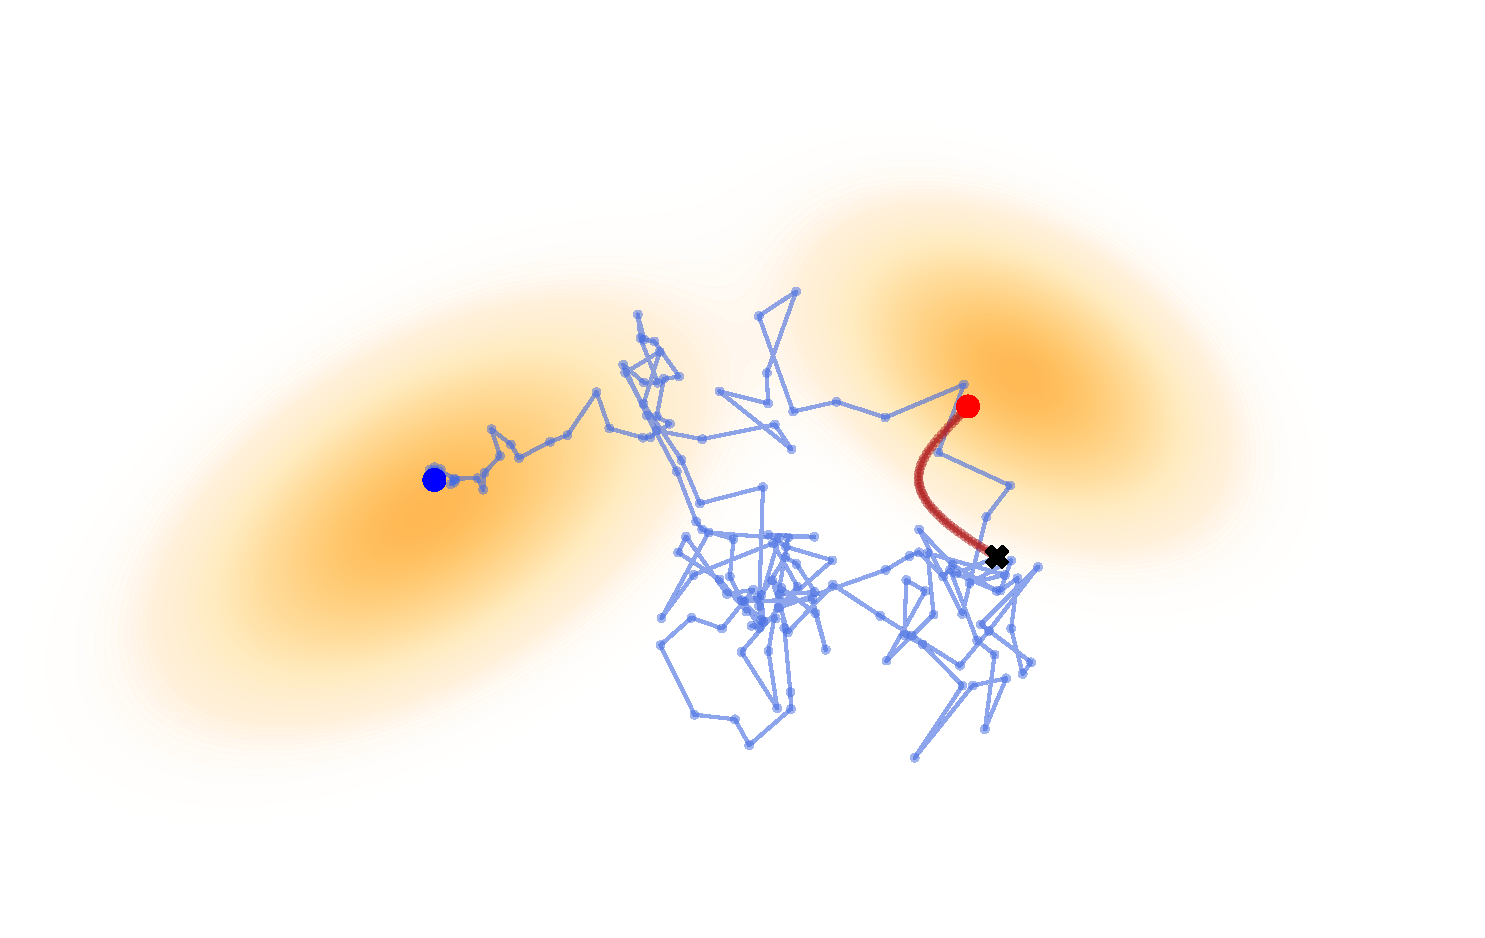
\includegraphics[width=\linewidth]{Images/PartB/sde_ode_trajectories.pdf}
    \vspace{-0.6cm}
    \caption{\textbfs{(2D) 从 Score SDE 采样的图示。} 前向 SDE 设计为 $\diff\rvx(t)=\sqrt{2t}\diff\rvw(t)$，有漂移 $\mathbf{f}\equiv\mathbf{0}$ 和扩散系数 $g(t)=\sqrt{2t}$ 开 $[0,T]$，演化出二模高斯混合 $p_0=p_{\mathrm{data}}$ 进入 $p_T\approx p_{\mathrm{prior}}:=\mathcal{N}(\mathbf{0},T^2\mathbf{I})$。显示的是反向时间 SDE 的采样轨迹（蓝色；通过以下方式求解） \Cref{eq:euler-maruyama}) 和 PF-ODE（红色；通过 \Cref{eq:euler-ode}）。从随机点开始 $\rvx_T\sim p_{\mathrm{prior}}$ （黑暗``$\times$'')，两条轨迹都朝着 $p_{\mathrm{data}}$ 如 $t\to 0$.
    \figcredit{由作者创建。}}
    \label{fig:sde_ode_trajectories}
\end{figure}


学习后 
\[
\mathbf{s}_{\bm{\phi}^\times} := \mathbf{s}_{\bm{\phi}^\times}(\rvx, t) \approx \nabla_{\rvx} \log p_t(\rvx),
\]
我们替换了棘手的预言机分数 $\nabla_{\rvx} \log p_t(\rvx)$ 在反向时间 SDE 中（\Cref{eq:sde_backward}) 和 PF-ODE (\Cref{eq:prob_ode_gt}) 与学习到的代理 $\mathbf{s}_{\bm{\phi}^\times}(\rvx, t)$。这种替换可以通过 SDE 或 ODE 进行易于处理的推理。为了清楚起见，我们将结果过程区分为 $\rvx^{\mathrm{SDE}}_{\bm{\phi}^\times}(t)$ 和 $\rvx^{\mathrm{ODE}}_{\bm{\phi}^\times}(t)$分别，但在后面的部分中将省略这种区别。\footnote{这是为了简化本小节之后的符号。}

\paragraph{经验反向时间 SDE。}
通过替换训练好的分数模型 $\mathbf{s}_{\bm{\phi}^\times}$ 为真实分数 \Cref{eq:sde_backward}，我们得到用于生成的参数化逆时SDE：
\begin{equation}\label{eq:sde_backward_sub}
    \diff \rvx^{\mathrm{SDE}}_{\bm{\phi}^\times}(t) = \left[\mathbf{f}\left(\rvx^{\mathrm{SDE}}_{\bm{\phi}^\times}(t), t\right) - g^2(t) \mathbf{s}_{\bm{\phi}^\times}\left(\rvx^{\mathrm{SDE}}_{\bm{\phi}^\times}(t), t\right) \right] \diff t + g(t) \diff \bar{\rvw}(t).
\end{equation}
为了生成样本，我们首先绘制一个初始值 $\rvx_T$ 来自先验分布 $p_{\mathrm{prior}}$ 然后数值求解 \Cref{eq:sde_backward_sub} 时间向后 $t=T$ 至 $t=0$。一个标准的数值求解器是 Euler-Maruyama 方法，它提供了离散更新规则：
\begin{equation}\label{eq:euler-maruyama}
\rvx_{t - \Delta t} \leftarrow \rvx_t - \left[ \mathbf{f}(\rvx_t, t) - g^2(t)  \mathbf{s}_{\bm{\phi}^\times}(\rvx_t, t) \right] \Delta t + g(t) \sqrt{\Delta t} \cdot \boldsymbol{\epsilon},
\end{equation}
其中 $\boldsymbol{\epsilon} \sim \mathcal{N}(\bm{0}, \mathbf{I})$ 和 $\Delta t > 0$ 是步长。

迭代此更新规则产生最终样本 $\rvx^{\mathrm{SDE}}_{\bm{\phi}^\times}(0)$。如果分数模型准确，则这些生成样本的分布，表示为 $p_{\bm{\phi}^\times}^{\mathrm{SDE}}(\cdot; 0)$，提供了接近真实数据分布的近似值\footnote{理论上，估计精度取决于之间的差异 $p_T$ 和 $p_{\mathrm{prior}}$ （通常可以忽略不计），模型训练误差和数值离散化误差~\citep{de2022convergence,wang2024evaluating}。我们在这里不追求正式的界限。}:
\[
p_{\bm{\phi}^\times}^{\mathrm{SDE}}(\cdot; 0) \approx p_{\mathrm{data}}(\cdot).
\]
确实，对于VP构建，DDPM采样方案
\Cref{eq:ddpm-sampling} 与上面的 Euler-Maruyama 离散化具有相同的连续时间反向 SDE 极限；看到 \Cref{sec:instances}.


\paragraph{经验 PF-ODE。}  
PF-ODE 定义了连续流连接 $p_{\mathrm{prior}}$ 和 $p_{\mathrm{data}}$，启用采样、编码和精确似然评估。以下部分提供了有关每个操作的更多详细信息。
\subparagraph{I. 使用 PF-ODE 采样。} 替换中的 oracle 分数 \Cref{eq:prob_ode_gt} 与 $\mathbf{s}_{\bm{\phi}^\times}$ 产生经验 PF-ODE：
\begin{equation}\label{eq:prob_ode_sub}
    \frac{\diff}{\diff t} \rvx^{\mathrm{ODE}}_{\bm{\phi}^\times}(t) = \mathbf{f}\left(\rvx^{\mathrm{ODE}}_{\bm{\phi}^\times}(t), t\right) - \frac{1}{2} g^2(t) \mathbf{s}_{\bm{\phi}^\times}\left(\rvx^{\mathrm{ODE}}_{\bm{\phi}^\times}(t), t\right).
\end{equation}
为了生成样本，我们首先绘制初始样本 $\rvx_T$ 根据先验分布， $p_{\mathrm{prior}}$。然后我们对 PF-ODE 进行数值求解 \Cref{eq:prob_ode_sub} 时间向后 $t=T$ 至 $t=0$。这个过程相当于近似积分：
\[
\rvx^{\mathrm{ODE}}_{\bm{\phi}^\times}(0) = \rvx_T + \int_T^0 \left[ \mathbf{f}\left(\rvx^{\mathrm{ODE}}_{\bm{\phi}^\times}(\tau), \tau\right) - \frac{1}{2} g^2(\tau) \mathbf{s}_{\bm{\phi}^\times}\left(\rvx^{\mathrm{ODE}}_{\bm{\phi}^\times}(\tau), \tau\right) \right] \mathrm{d}\tau.
\]
求解该积分会产生最终样本， $\rvx^{\mathrm{ODE}}_{\bm{\phi}^\times}(0)$。通过这个确定性过程生成的样本分布，表示为 $p_{\bm{\phi}^\times}^{\mathrm{ODE}}(\cdot; 0)$，提供数据分布的近似值，使得 $p_{\bm{\phi}^\times}^{\mathrm{ODE}}(\cdot; 0) \approx p_{\mathrm{data}}$。让 $\Delta t > 0$ 表示离散化步长。标准数值积分方法是欧拉方法，它估计
\[
\mathbf{f}(\rvx_\tau, \tau) - \frac{1}{2} g^2(\tau)  
\mathbf{s}_{\bm{\phi}^\times}(\rvx_\tau, \tau) \approx \mathbf{f}(\rvx_t, t) - \frac{1}{2} g^2(t)  
\mathbf{s}_{\bm{\phi}^\times}(\rvx_t, t), \quad \tau \in [t-\Delta t, t],
\]
导致以下更新规则：
\begin{equation}\label{eq:euler-ode}
\rvx_{t - \Delta t} \leftarrow \rvx_t -
\left[ \mathbf{f}(\rvx_t, t) - \frac{1}{2} g^2(t)  
\mathbf{s}_{\bm{\phi}^\times}(\rvx_t, t) \right] \Delta t.
\end{equation}


这种联系使我们能够通过以下核心洞察来重新构建生成过程：
\msg{洞察力}{Generation $\Leftrightarrow$ ODE/SDE Solving}{从扩散模型中采样基本上等同于求解相应的概率流 ODE 或反向时间 SDE。}

这种等价性为扩散模型的采样速度慢提供了清晰的解释，如问题中提出的~\ref{ques:dm-sampling-slow}。生成过程需要大量计算，因为这些微分方程的数值求解器本质上是迭代的，通常需要许多步骤才能准确地近似解轨迹\footnote{例如，DDPM 和 Score SDE 通常使用 $1,000$ 生成的功能评估。}。然而，PF-ODE 公式也有优势，因为它允许我们利用有关加速数值求解器的大量文献。探索这些技术来加速扩散模型采样是主要关注点 \Cref{ch:solvers}.

\subparagraph{II。使用 PF-ODE.} 进行反演 正如所讨论的，与 SDE 的情况不同，我们可以及时求解相同的 \Cref{eq:prob_ode_sub} 正向（从 $0$ 到 $T$）和反向（从 $T$ 到 $0$）。正向求解时，ODE 流程将数据映射到所有 $t \in [0,T]$ 中的（噪声）潜在表示，这起到了编码器的作用。这一概念使强大的应用程序能够实现可控生成，例如图像翻译和编辑以及~\citep{mokady2023null,su2022dual}。

\subparagraph{三．通过 PF-ODE.} 进行对数似然评估
概率流 ODE 还可以用来计算数据样本的似然。
回想一下 \Cref{eq:instant-change-of-var}，对于 ODE，
沿轨迹的对数密度由其速度的散度决定
场。

对于学习到的 PF-ODE，定义
\[
\rvv_{\bm{\phi}^\times}(\rvx,t)
:=
\rvf(\rvx,t)
-\frac{1}{2}g^2(t)\rvs_{\bm{\phi}^\times}(\rvx,t).
\]
如果$\rvx(t)$按照
\[
\frac{\diff}{\diff t}\rvx(t)
=
\rvv_{\bm{\phi}^\times}(\rvx(t),t),
\]
那么它的对数密度满足
\[
\frac{\diff}{\diff t}
\log p^{\textup{ODE}}_{\bm{\phi}^\times}(\rvx(t);t)
=
-\nabla_{\rvx}\cdot
\rvv_{\bm{\phi}^\times}(\rvx(t),t).
\]

为了计算观测样本 $\rvx_0$ 的似然，我们沿概率流 ODE 积分
从 $t=0$ 转发到 $t=T$，将 $\rvx_0$ 映射到
模型密度是易于处理的先验。我们可以同时追踪
通过定义对数密度变化
\[
\delta(t)
:=
\log p^{\textup{ODE}}_{\bm{\phi}^\times}(\rvx(t);t)
-
\log p^{\textup{ODE}}_{\bm{\phi}^\times}(\rvx_0;0).
\]
因此，可以计算 $\delta(0)=0$ 以及状态和对数密度变化
一起通过
\begin{align}\label{eq:score-sde-likelihood}
\frac{\diff}{\diff t}
\begin{bmatrix}
\rvx(t)\\
\delta(t)
\end{bmatrix}
=
\begin{bmatrix}
\rvv_{\bm{\phi}^\times}(\rvx(t),t)\\
-\nabla_{\rvx}\cdot
\rvv_{\bm{\phi}^\times}(\rvx(t),t)
\end{bmatrix},
\qquad
\begin{bmatrix}
\rvx(0)\\
\delta(0)
\end{bmatrix}
=
\begin{bmatrix}
\rvx_0\\
0
\end{bmatrix}.
\end{align}

集成到$t=T$后，终端密度为
$p_{\mathrm{prior}}(\rvx(T))$。因此，
\[
\log
p^{\textup{ODE}}_{\bm{\phi}^\times}(\rvx_0;0)
=
\log p_{\mathrm{prior}}(\rvx(T))
-
\delta(T).
\]
等价地，
\[
\log
p^{\textup{ODE}}_{\bm{\phi}^\times}(\rvx_0;0)
=
\log p_{\mathrm{prior}}(\rvx(T))
+
\int_0^T
\nabla_{\rvx}\cdot
\rvv_{\bm{\phi}^\times}(\rvx(t),t)
\,\diff t.
\]
因此，用于生成和反演的相同 PF-ODE 还提供了
用于似然评估的连续变量变换公式。




\newpage

\section{两类常用的 SDE}\label{sec:instances}

\citet{song2020score} 按方差随时间的变化，将漂移项 $\rvf(\rvx, t)$ 和扩散系数 $g(t)$ 的选择划分为三类。这里介绍两种常用情形，即\emph{方差爆炸}（VE）SDE 和\emph{方差保持}（VP）SDE。噪声调度可以自行设计，它的选择会显著影响实际效果。
表~\ref{tb:sde_instances} 总结了这两个SDE 实例。
\begin{table}[th]
  \caption{远期SDE摘要}
  \small
  \centering
  \resizebox{\textwidth}{!}{
  \begin{tabular}{cccc}
     \toprule
    
         & \textbfs{VE SDE} & \textbfs{VP SDE} \\
       \midrule
    $\mathbf{f}(\rvx, t)$ & $\mathbf{0} $ & $-\frac{1}{2}\beta(t)\rvx$ \\
      $g(t)$ & $\sqrt{\frac{\diff \sigma^2(t)}{\diff t}}$ 
      
       & $\sqrt{\beta(t)}$ \\

    SDE & $\diff\rvx(t) =  g(t) \diff\rvw(t)$ & $\diff\rvx(t) = -\frac{1}{2}\beta(t) \rvx(t) \diff t + \sqrt{\beta(t)} \diff\rvw(t)$ \\
   \midrule
     $p_t(\rvx_t|\rvx_0)$ & $        \mathcal{N}\left(\rvx_t ; \rvx_0, \left(\sigma^2(t) - \sigma^2(0)\right)\rmI\right)$ & $ \mathcal{N}\left(\rvx_t ; \rvx_0 e^{-\frac{1}{2}\int_{0}^{t} \beta(\tau)\diff \tau}, \rmI - \rmI e^{-\int_{0}^{t} \beta(\tau)\diff \tau}\right)$ \\
   
     $p_{\mathrm{prior}}$ & $ \mathcal{N}(\bm{0}, \sigma^2(T)\rmI)$ & $\mathcal{N}(\bm{0}, \rmI)$ \\
 \bottomrule
  \end{tabular}
  }
  \label{tb:sde_instances}
\end{table}\subsection{VE SDE}
VE SDE 具有以下组件：
\begin{itemize}
    \item \textbfs{漂移项：} 零漂移项 $\mathbf{f}=\bm{0}$。
    \item \textbfs{扩散系数：} $g(t)=\sqrt{\frac{\diff \sigma^2(t)}{\diff t}}$ 其中函数$\sigma(t)$。
\end{itemize}
前向 SDE 的形式如下：
\begin{equation}\label{eq:vesde}
    \diff\rvx(t) =  \sqrt{\frac{\diff \sigma^2(t)}{\diff t}} \diff\rvw(t).
\end{equation} 
同样，\Cref{subsec:scoresde-perturbation-kernel} 的结果暗示了 VE SDE 的扰动内核，并建议选择适当的先验分布：
\begin{itemize}
    \item \textbfs{扰动内核：}
\begin{align*}
        p_t(\rvx_t | \rvx_0) &= \mathcal{N}\left(\rvx_t ; \rvx_0, \left(\sigma^2(t) - \sigma^2(0)\right)\rmI\right) 
\end{align*}
    \item \textbfs{先验分布：} 假设$\sigma(t)$ 是$t \in [0,T]$ 和$\sigma^2(T) \gg \sigma^2(0)$ 的增函数。先验分布由下式给出：
    \[
    p_{\mathrm{prior}} := \mathcal{N}(\bm{0}, \sigma^2(T)\rmI).
    \]
\end{itemize}

VE SDE 的典型实例是 NCSN，其设计如下：
\[
\sigma(t):=\sigma_{\textup{min}}\left(\frac{\sigma_{\textup{max}}}{\sigma_{\textup{min}}} \right)^t,\quad \text{for } t\in(0,1],
\]
其中 $\sigma_{\textup{min}}$ 和 $\sigma_{\textup{max}}$ 是预先指定的常数。即，方差序列被设计为几何序列。由此，NCSN 被视为 VE SDE 的离散化版本，如 \Cref{subsec:scoresde-motivation} 中所述。

































\subsection{VP SDE}
令 $\beta\colon [0,T] \rightarrow \mathbb{R}_{\geq 0 }$ 为 $t$ 的非负函数。 VP SDE 由以下组件定义：
\begin{itemize}
    \item \textbfs{漂移 术语：} $\mathbf{f}(\rvx, t) = -\frac{1}{2}\beta(t)\rvx$ 给出的线性漂移。
    \item \textbfs{扩散系数：} $g(t) = \sqrt{\beta(t)}$。
\end{itemize}
因此，前向SDE可表示为：
\begin{align}\label{eq:forward-linear-sde}
\diff\rvx(t) = -\frac{1}{2}\beta(t) \rvx(t) \diff t + \sqrt{\beta(t)} \diff\rvw(t).
\end{align}

使用 \Cref{subsec:scoresde-perturbation-kernel} 的结果，我们可以推导出 VP SDE 的扰动内核并选择适当的先验分布：
\begin{itemize}
    \item \textbfs{扰动内核：}
    \[
    p_t(\rvx_t|\rvx_0) = \mathcal{N}\left(\rvx_t ; \rvx_0 e^{-\frac{1}{2}\int_{0}^{t} \beta(\tau)\diff \tau}, \rmI - \rmI e^{-\int_{0}^{t} \beta(\tau)\diff \tau}\right).
    \]
    \item \textbfs{先前分发：} $p_{\mathrm{prior}} := \mathcal{N}(\bm{0}, \rmI)$。
\end{itemize}
我们注意到，由于扰动核是具有已知均值和协方差的高斯函数，因此我们可以应用 \Cref{eq:gaussian-score} 来计算其分数函数。

VP SDE 的一个典型示例是 DDPM，其中噪声表 $\beta(t)$ 定义为：
\[
\beta(t) := \beta_{\textup{min}} + t(\beta_{\textup{max}} - \beta_{\textup{min}}), \quad \text{for all } t \in [0,1].
\]
这里，$\beta_{\textup{min}}$和$\beta_{\textup{max}}$是预定义的常量。由此，DDPM 可以解释为 VP SDE 的离散化，如 \Cref{subsec:scoresde-motivation} 中所讨论的。






\subsection{（选读）扰动核如何 
$ p_t(\rvx_t|\rvx_0) $ 派生？}\label{subsec:scoresde-perturbation-kernel}
如果正向 SDE \Cref{eq:sde_forward} 中的漂移项在 $\rvx$ 中是线性的，则采用以下形式
\begin{align*}
    \rvf(\rvx, t) = f(t) \rvx,
\end{align*}
对于某些标量值、时间相关函数 $f(t) \in \mathbb{R}$，则 \Cref{eq:sde_forward} 变为线性 SDE：
\[
\diff\rvx(t) = f(t)\rvx(t) \diff t + g(t) \diff\rvw(t).
\]


即使初始分布 $p_{\mathrm{data}}$ 是非高斯分布，漂移的线性也确保条件过程保持高斯分布。特别是，对于 $t>0$，转换内核接受以下形式：
\[
p_t( \rvx_t | \rvx_0 ) = \mathcal{N} \left( \rvx_t;  \rvm(t),  P(t) \mathbf{I}_D \right),
\]
其中 $\rvx_0 \sim p_{\mathrm{data}}$ 和 $\rvm(t) \in \mathbb{R}^D$、$P(t)\in\mathbb{R}_{\ge 0}$ 表示给定 $\rvx_0$ 的条件均值和（标量）方差，定义为：
\[
\rvm(t) = \mathbb{E} \left[\rvx_t | \rvx(0) = \rvx_0\right], \qquad
P(t) \mathbf{I}_D = \operatorname{Cov} \left[\rvx_t | \rvx(0) = \rvx_0\right].
\]

这些第一和第二时刻根据以下 ODE 演化~\citep{sarkka2019applied}:
\begin{align}\label{eq:mean-var-evolution}
\begin{aligned}
    \frac{\diff \rvm(t)}{\diff t} &= f(t) \rvm(t), \\
    \frac{\diff P(t)}{\diff t} &= 2f(t) P(t) + g^2(t),
\end{aligned}
\end{align}
前提是初始平均值 $\rvm(0)$ 和方差 $P(0)$ 是有限的。由于两个 ODE 都是线性的，因此它们可以通过积分因子方法获得封闭式解。给定初始条件 $\rvx_0$，均值和方差演变为
\begin{align}\label{eq:mean-var-solution}
    \rvm(t) = \mathcal{E}(0  \to  t) \rvx_0, 
\qquad 
P(t) = \int_{0}^{t} \mathcal{E}^{2}(s  \to  t)  g(s)^{2} \diff s,
\end{align}
与 $\rvm(0)=\rvx_0$ 和 $P(0)=0$。这里 $\mathcal{E}(s  \to  t)$ 表示指数积分因子
\[
\mathcal{E}(s  \to  t) := \exp \left(\int_{s}^{t} f(u) \diff u\right),
\]
捕捉时间漂移的累积效应 $s$ 至 $t$。因此，转移核 $p_t(\rvx_t | \rvx_0)$ 也允许封闭式表达式。我们推迟了条件协方差的论证 $p_t(\rvx_t |\rvx_0)$ 是各向同性的，即 
$\operatorname{Cov}[\rvx_t | \rvx_0] = P(t) \mathbf I_D$ 下一个 $D$具有独立坐标和扩散的维纳过程 $g(t)\mathbf I_D$，以及推导 \Cref{eq:mean-var-evolution}, 至 \Cref{subsec:rigorous-proof-linear-sde}，依赖于 Itô 微积分。


\exm{VE SDE 的转换内核}{在 VE SDE 的特殊情况下： $\rvf \equiv 0$ 和 $g(t) = \sqrt{\frac{\diff \sigma^2(t)}{\diff t}}$，SDE 解的均值和协方差演变如下。

\proofparagraph{意思是。}
\[
\frac{\diff \rvm(t)}{\diff t} = 0, 
\quad \text{with} \quad \rvm(0) = \rvx_0
 \Longrightarrow 
\rvm(t) = \rvx_0.
\]

\proofparagraph{方差。}
\[
\frac{\diff P(t)}{\diff t} = \frac{\diff \sigma^2(t)}{\diff t},
\quad \text{with} \quad P(0) = 0
 \Longrightarrow 
P(t) = \sigma^2(t) - \sigma^2(0).
\]
因此
\[
p_t(\rvx_t | \rvx_0)=\mathcal{N} \left(\rvx_t;  \rvx_0,  \big(\sigma^2(t)-\sigma^2(0)\big)\mathbf{I}_D\right).
\]
}

\exm{VP SDE 的转换内核}{在带有漂移的 VP SDE 情况下 $\rvf(\rvx, t) = -\tfrac{1}{2}\beta(t) \rvx$ 和扩散 $g(t) = \sqrt{\beta(t)}$:

\proofparagraph{平均值 $\rvm(t)$.}
\[
\frac{\diff \rvm}{\diff t}
= -\frac{1}{2}\beta(t) \rvm(t),
\quad
B(t) \coloneqq \int_{0}^{t} \beta(s) \diff s,
\quad
\rvm(t) = e^{-\frac{1}{2}B(t)} \rvx_0.
\]

\proofparagraph{方差 $P(t)$.} 方差满足
\[
\frac{\diff P}{\diff t} = -\beta(t) P(t) + \beta(t).
\]
应用积分因子 $e^{B(t)}$ 与 $B(t) = \int_0^t \beta(s) \diff s$，我们得到
\[
\frac{\diff}{\diff t} \left[P(t)e^{B(t)}\right] = \beta(t) e^{B(t)}.
\]
两边积分得出
\[
P(t) = 1 - e^{-B(t)}.
\]
因此协方差是各向同性的
\[
\rmP(t) = P(t) \mathbf I_D = \bigl(1 - e^{-B(t)}\bigr)\mathbf I_D.
\]

\proofparagraph{最终封闭式转换内核。}
\[
p_t(\rvx_t|\rvx_0)
= \mathcal{N} \left(
   \rvx_t; 
   \underbrace{e^{-\frac{1}{2} B(t)} \rvx_0}_{\rvm(t)}, 
   \underbrace{\big(1 - e^{-B(t)}\big)\mathbf{I}_D}_{P(t)\mathbf{I}_D}
\right),
\quad
B(t) = \int_0^t \beta(s) \diff s.
\]
}

\clearpage
\newpage


\section{\texorpdfstring{从累积扰动核看分数 SDE}{从累积扰动核看分数 SDE}}
\label{sec:variational-perspective}

DDPM 和 Score SDE 通常是通过指定如何及时在本地添加噪声来引入的：通过离散前向转换
$p(\rvx_t|\rvx_{t-\Delta t})$ 在DDPM中，或者通过Score SDE中的连续时间SDE。然而，对于训练来说，一个特别有用的对象是
\emph{累积扰动核}
\[
p_t(\rvx_t|\rvx_0),
\]
描述了时间的分布 $t$ 直接以原始数据样本为条件。这正是 DDPM 和连续时间去噪目标中自然出现的形式
\Cref{eq:ddpm-mean-loss,eq:conti-dsm_loss-real}.

这提出了一个互补的观点：而不是从局部噪声注入开始，然后推导 $p_t(\rvx_t|\rvx_0)$，我们可以直接指定累积扰动核。对于下面考虑的线性高斯过程，允许的累积核确定相应的线性 SDE，反之亦然。这种观点使每个时间的信号和噪声量变得明确，直接与实际训练目标联系起来，并且还将为流匹配的概率路径观点提供一个有用的桥梁。 \Cref{ch:flow-based}.

\begin{figure}[th!]
    \centering
    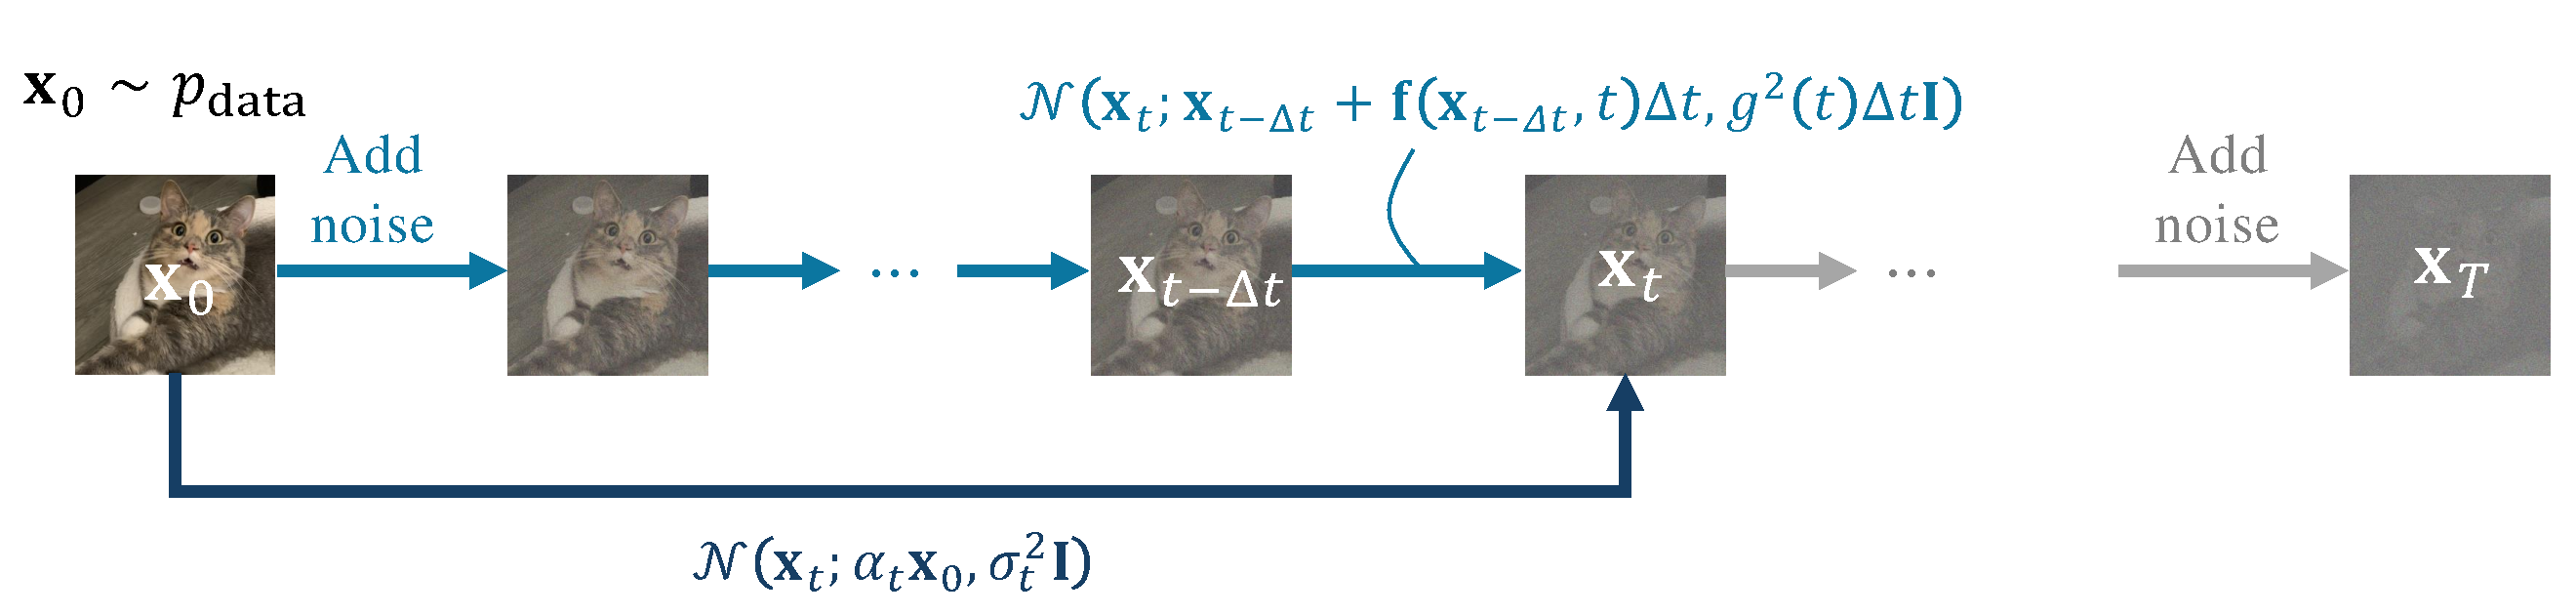
\includegraphics[width=\linewidth]{Images/PartB/vdm-sde.pdf}
    \caption{\textbfs{同一仿射前向过程的两个视图。}
    对于可接受的仿射扩散方案，通过连续时间线性 SDE 进行增量噪声注入，并直接指定累积扰动核 \Cref{eq:forward_kernel} 描述相同的条件分布 $p_t(\rvx_t|\rvx_0)$.
    \figcredit{由作者创建。}}
    \label{fig:vdm-sde}
\end{figure}

\paragraph{通用仿射前向过程 $p_t(\rvx_t|\rvx_0)$.}
我们首先定义累积前向扰动内核
\begin{equation}\label{eq:forward_kernel}
p_t(\rvx_t|\rvx_0)
:=
\mathcal{N}\bigl(
\rvx_t;
\alpha_t\rvx_0,
\sigma_t^2\mathbf{I}
\bigr),
\end{equation}
其中 $\rvx_0\sim p_{\mathrm{data}}$, 和 $\alpha_t$ 和 $\sigma_t$ 是非负标量函数 $t\in[0,T]$。在标准前向扩散设置中，我们采用
\[
\alpha_0=1,
\qquad
\sigma_0=0,
\]
以便该过程完全从数据开始，并假设
$\alpha_t>0$ 和 $\sigma_t>0$ 用于 $t\in(0,T]$ 每当使用相应的比率时。等价地，样本来自 \Cref{eq:forward_kernel} 可以写成
\[
\rvx_t
=
\alpha_t\rvx_0
+
\sigma_t\bm{\epsilon},
\qquad
\bm{\epsilon}\sim\mathcal{N}(\mathbf{0},\mathbf{I}).
\]

这个简单的形式包括几个熟悉的概率路径：
\begin{itemize}
    \item \textbfs{VE（NCSN）：}
    $\alpha_t\equiv1$，带有噪声标度 $\sigma_t$ 随时间增加；
    \item \textbfs{副总裁（DDPM）：}
    $\alpha_t^2+\sigma_t^2=1$;
    \item \textbfs{线性高斯插值：}
    $\alpha_t=1-t$ 和 $\sigma_t=t$ 开 $t\in[0,1]$，对应于以数据噪声时间约定编写时在流匹配和整流流中使用的熟悉的线性路径。
\end{itemize}

\subsection{与 Score SDE 的连接}
对于Score SDE，指定累积扰动核通常更直观 $p_t(\rvx_t|\rvx_0)$ 先恢复相应的SDE系数，而不是从漂移项和扩散项开始求解矩的ODE（参见 \Cref{subsec:scoresde-perturbation-kernel}）。对于可接受的仿射调度，相应的前向 SDE 采用线性-in-$\rvx$ 表格中 \Cref{eq:forward-linear-sde}:
\begin{align*}
    \diff \rvx(t)
    =
    \underbrace{f(t)\rvx(t)}_{\rvf(\rvx(t),t)}
    \diff t
    +
    g(t)\diff\rvw(t),
\end{align*}
其中 $f,g\colon[0,T]\rightarrow\mathbb{R}$ 是时间的实值函数。

系数 $f(t)$ 和 $g(t)$ 可以从分析中恢复
$\alpha_t$ 和 $\sigma_t$。重要的是，并非所有选择
$\alpha_t$ 和 $\sigma_t$ 定义有效扩散：隐含扩散方差 $g^2(t)$ 必须保持非负。同样，在这种线性高斯设置中，信噪比
$\alpha_t^2/\sigma_t^2$ 不能随时间增加。下面的引理使这种关系变得精确。

\lemp{前向扰动内核 $\Leftrightarrow$ 线性 SDE}{forward-sde}{
假设 $\alpha_0=1$, $\sigma_0=0$，还有 $\alpha_t>0$ 和
$\sigma_t>0$ 可微分 $t\in(0,T]$。定义
$\lambda_t:=\log\tfrac{\alpha_t}{\sigma_t}$。给定前向扰动核
\[
\rvx_t=\alpha_t\rvx_0+\sigma_t\beps,
\qquad
\beps\sim\mathcal N(\mathbf 0,\rmI),
\]
存在对应的线性SDE
\[
\diff \rvx(t)=f(t)\rvx(t)\diff t+g(t)\diff\rvw(t)
\]
具有相同的条件内核
$p_t(\rvx_t|\rvx_0)
=\mathcal N(\rvx_t;\alpha_t\rvx_0,\sigma_t^2\rmI)$
当且仅当系数
\begin{align}\label{eq:kernel-sde-equiv}
\begin{aligned}
f(t)
&=\frac{\diff}{\diff t}\log\alpha_t,\\
g^2(t)
&=\frac{\diff\sigma_t^2}{\diff t}
-2\frac{\diff}{\diff t}\log\alpha_t\,\sigma_t^2
=-2\sigma_t^2\frac{\diff}{\diff t}\lambda_t
\end{aligned}
\end{align}
满足 $g^2(t)\geq0$ 用于 $t\in(0,T]$。等价地， $\lambda_t$ 必须是非递增的。相反，如果线性 SDE 具有条件核
$\mathcal N(\rvx_t;\alpha_t\rvx_0,\sigma_t^2\rmI)$ 与
$\alpha_t>0$ 和 $\sigma_t>0$，则其系数必然满足
\Cref{eq:kernel-sde-equiv}.
}{
来自 \Cref{subsec:scoresde-perturbation-kernel}，通过匹配均值和协方差 ODE 得出结果
$\rvm'(t)=f(t)\rvm(t)$ 和
$\rmP'(t)=2f(t)\rmP(t)+g^2(t)\rmI$
与 $\rvm(t)=\alpha_t\rvx_0$ 和
$\rmP(t)=\sigma_t^2\rmI$.
}

\rmkb{使终端条件分布独立于 $\rvx_0$ 并且等于规定的高斯先验，我们需要
$\alpha_T=0$ 和 $\sigma_T^2$ 等于先验方差。自从
\[
\alpha_t
=
\exp\Big(\int_0^t f(u)\diff u\Big),
\]
实现 $\alpha_T=0$ 在有限的终端时间需要
\[
\int_0^T f(u)\diff u=-\infty.
\]
因此，漂移引起的收缩必定在接近终止时间时变得奇异；特别是， $f$ 无法保持限制 $[0,T]$。扩散系数与规定方差相关：
\[
g^2(t)
=
(\sigma_t^2)'
-
2\frac{\alpha_t'}{\alpha_t}\sigma_t^2.
\]
对于通常的定期时间表，其中
$\sigma_t^2$ 接近有限非零终端方差，
$(\sigma_t^2)'$ 仍然有界，并且
$\alpha_t'/\alpha_t\to-\infty$，这也给出了
\[
g^2(t)\to\infty
\qquad\text{as }t\to T.
\]
更一般地说，的精确行为 $g(t)$ 取决于所选的时间表。如果 $f$ 和 $g$ 保持有限区间上的界限 $[0,T]$，那么
$\alpha_T>0$，所以在有限的情况下不可能发生精确的遗忘 $T$。因此，在实践中，人们会选择一个最终时间，在这个时间里，剩余依赖性 $\rvx_0$ 可以忽略不计并且 $p_T\approx p_{\mathrm{prior}}$，或考虑无限时间公式，其中 $\alpha_t\to0$
渐近。
}


根据上述引理，通过带有系数的线性 SDE 指定增量噪声注入 $f(t)$ 和 $g(t)$ 数学上等价于用参数定义扰动核 $\alpha_t$ 和 $\sigma_t$。在扩散模型文献中，这两种观点可以互换使用。因此，我们得出结论：
\msg{观察}{}{
对于有效的仿射扩散计划，两种描述是等效的：我们可以指定累积的扰动内核
$p_t(\rvx_t|\rvx_0)$ 通过 $\alpha_t$ 和 $\sigma_t$，或者通过指定对应的线性SDE $f(t)$ 和 $g(t)$.
}


\subsection{与基于变分的扩散模型的连接}\label{subsec:connection-vdm}
我们重新审视 DDPM 的核心恒等式，通过贝叶斯规则导出：
\begin{align}\label{eq:ddpm-reverse-condition-kernel}
    p(\rvx_{t-\Delta t}|\rvx_t, \rvx) = p(\rvx_t|\rvx_{t-\Delta t}) \cdot \frac{p_{t-\Delta t}(\rvx_{t-\Delta t}|\rvx)}{p_t(\rvx_t|\rvx)},
\end{align}
对于任何 $\rvx$ （通常 $\rvx\sim p_{\mathrm{data}}$）。这个反向条件 $ p(\rvx_{t-\Delta t} | \rvx_t, \rvx) $ 是建模的核心，可实现易于处理的训练目标和高效的采样。尽管 DDPM 通常定义增量内核 $p(\rvx_t|\rvx_{t-\Delta t})$ 一、累积转变 $p_t(\rvx_t|\rvx_0)$ 通常提供更具可解释性和实用性的公式，特别是对于先验和损耗设计。

\paragraph{导出转换内核。}
我们现在将其扩展到连续时间设置。让 $0 \leq t < s \leq T$ 是两个（连续的）时间点。给定扰动核 $p_t(\rvx_t|\rvx_0)$，我们可以计算相反的条件 $p(\rvx_t|\rvx_s, \rvx)$ 对于任何 $\rvx$ 通过申请 \Cref{eq:ddpm-reverse-condition-kernel}\footnote{通过处理，该恒等式自然延伸到连续时间 $s$ 一般时间较早。}，使用前向转移核 $p(\rvx_s|\rvx_t)$ 作为中间体。下面的引理总结了这个推导，扩展了引理~\ref{ddpm-reverse-kernel} 无需假设 $\alpha_t^2 + \sigma_t^2 = 1$.

\lemp{反向条件转换内核}{reverse-kernel}{
让 $0 \leq t < s \leq T$。反过来 \emph{有条件} 过渡内核是：
\begin{equation*}
    p(\rvx_t|\rvx_s, \rvx) = \mathcal{N}\left(\rvx_t; \bm{\mu}(\rvx_s, \rvx; s, t), \sigma^2(s, t) \bfI\right),
\end{equation*}
其中
\begin{align}\label{eq:p_backward_mean_var}
\begin{aligned}
    \bm{\mu}(\rvx_s, \rvx; s, t) := \frac{\alpha_{s|t} \sigma_t^2}{\sigma_s^2} \rvx_s + \frac{\alpha_t \sigma^2_{s|t}}{\sigma_s^2} \rvx, \quad
    \sigma^2(s, t) := \sigma^2_{s|t} \frac{\sigma_t^2}{\sigma_s^2}.
\end{aligned}
\end{align}
在这里， $\alpha_{s|t}$ 和 $\sigma_{s|t}$ 定义为：
\begin{equation*}
    \alpha_{s|t} := \frac{\alpha_s}{\alpha_t}, \qquad \sigma^2_{s|t} := \sigma_s^2 - \alpha_{s|t}^2 \sigma_t^2.
\end{equation*}
}{
我们首先计算前向过渡内核：
\begin{equation}\label{eq:zt_given_zs}
    p(\rvx_s|\rvx_t) = \mathcal{N}\left(\rvx_s; \alpha_{s|t} \rvx_t, \sigma^2_{s|t} \bfI\right).
\end{equation}
反向转移核遵循贝叶斯规则，并且由于所有涉及的分布都是高斯分布，因此可以通过直接计算得出结果。欲了解更多详情，请参阅附录 A \citep{kingma2021variational}.
}


虽然 $p(\rvx_{t + \Delta t}|\rvx_t)$ 和 $p_t(\rvx_t|\rvx_0)$ 理论上是等价的， $p_t(\rvx_t|\rvx_0)$ 通常扮演更核心的角色。逐步过渡在 \Cref{eq:zt_given_zs} 主要用于获得封闭形式的反向转移核。近期作品~\citep{kingma2021variational} 因此赞成直接指定 $p_t(\rvx_t|\rvx_0)$ 因其清晰性和可解释性。



\paragraph{逆向过程建模、训练和采样。}  
训练目标（ELBO \Cref{eq:ddpm-elbo}) 以及中介绍的建模框架 \Cref{sec:ddpm} 在我们的通用设置下仍然适用。为了清楚起见，我们采用 $\rvx$-预测公式，表示为 $\rvx_{\bm{\phi}}(\rvx_s, s)$，以下~\citet{kingma2021variational}。然而，等效的 $\beps$-预测视角，表示为 $\bm{\epsilon}_{\bm{\phi}}(\rvx_s, s)$，由于以下关系也有效（如 \Cref{eq:ddpm-clean-noise})
\[
\rvx_s = \alpha_s \rvx_{\bm{\phi}}(\rvx_s, s) + \sigma_s \bm{\epsilon}_{\bm{\phi}}(\rvx_s, s),\quad \text{for any given } \rvx_s \sim q_s.
\]

\subparagraph{建模和扩散损失 $\mathcal{L}_{\text{diffusion}}$.}  
与DDPM类似，条件分布 $p(\rvx_t|\rvx_s, \rvx)$ 在 \Cref{eq:p_backward_mean_var} 激励更换干净信号 $\rvx$ 具有可学习的预测器 $\rvx_{\bm{\phi}}(\rvx_s, s)$，产生以下形式的参数化逆向模型：
\begin{align}\label{eq:general-ddpm-sampling}
    p_{\bm{\phi}}(\rvx_t | \rvx_s) := \mathcal{N}\left(\rvx_t; \bm{\mu}_{\bm{\phi}}(\rvx_s, s, t), \sigma^2(s,t) \mathbf{I}\right),
\end{align}
平均值参数化为：
\[
    \bm{\mu}_{\bm{\phi}}(\rvx_s, s, t) = \frac{\alpha_{s|t} \sigma_t^2}{\sigma_s^2} \rvx_s + \frac{\alpha_t \sigma_{s|t}^2}{\sigma_s^2} \rvx_{\bm{\phi}}(\rvx_s, s).
\]
给定中的前向转移核 \Cref{eq:forward_kernel}，KL 散度 $\mathcal{L}_{\text{diffusion}}(\rvx; \bm{\phi})$ 减少为加权回归损失：
\begin{align}
\begin{aligned}
    \label{eq:snr-kl}
    \mathcal{D}_{\text{KL}}\big(p(\rvx_t|\rvx_s, \rvx_0)  \| p_{\bm{\phi}}(\rvx_t|\rvx_s)\big)  
    &= \frac{1}{2\sigma^2(s,t)} \left\| \bm{\mu}(\rvx_s, \rvx_0; s,t) - \bm{\mu}_{\bm{\phi}}(\rvx_s, s, t) \right\|_2^2 \\
    &= \frac{1}{2} \big(\text{SNR}(t) - \text{SNR}(s)\big) \left\| \rvx_0 - \rvx_{\bm{\phi}}(\rvx_s, s) \right\|_2^2,
\end{aligned}
\end{align}
其中 $\rvx_s = \alpha_s\rvx_0 + \sigma_s\bm{\epsilon}$，与 $\rvx_0 \sim p_{\mathrm{data}}$, $\bm{\epsilon} \sim \mathcal{N}(\bm{0}, \rmI)$, 和 $\text{SNR}(s) := \alpha_s^2 / \sigma_s^2$ 表示该时刻的信噪比 $s$.


\rmkb{
在 \citep{kingma2021variational}，作者研究了连续时间极限 \Cref{eq:snr-kl} 如 $t \to s$，产生：
\begin{align*}
\mathcal{L}_{\text{VDM}}^\infty(\rvx_0) 
= -\frac{1}{2}  \mathbb{E}_{s, \bm{\epsilon} \sim \mathcal{N}(\bm{0}, \bfI)}  \text{SNR}'(s)  \big\| \rvx_0 - \rvx_{\bm{\phi}}(\rvx_s, s) \big\|_2^2.
\end{align*}
此设置还引入了可学习的噪声表，虽然它概括了连续数据之外的内容，但此类扩展超出了我们当前讨论的范围。
}

\subparagraph{采样。}  
采样过程与使用参数化内核的 DDPM 类似 \Cref{eq:general-ddpm-sampling}:
\begin{align}\label{eq:general-ddpm-sampling-discrete}
    \rvx_t = \underbrace{\frac{\alpha_{s|t} \sigma_t^2}{\sigma_s^2} \rvx_s + \frac{\alpha_t \sigma_{s|t}^2}{\sigma_s^2} \rvx_{\bm{\phi}^\times}(\rvx_s, s)}_{\bm{\mu}_{\bm{\phi}^\times}(\rvx_s, t, s)} + \sigma_{s|t} \frac{\sigma_t}{\sigma_s} \bm{\epsilon}_s,\quad  \bm{\epsilon}_s \sim \mathcal{N}(\bm{0}, \rmI).
\end{align}



\clearpage
\newpage

\section{（选读）用边缘化与贝叶斯公式理解福克尔-普朗克方程和反向时间 SDE}\label{eq:heuristic-fpe-sde}
在本节中，我们从概率角度介绍 福克尔-普朗克方程和反向时间 SDE 的结构。通过利用边缘化技巧和贝叶斯规则等基本工具，我们阐明了随机过程的统计公式与其相应的微分方程之间的联系。我们强调，这里提出的“推导”不是数学上严格的证明，而是旨在传达潜在联系的启发式论证。


\subsection{来自转移核边缘化的 福克尔-普朗克方程}\label{subsec:fpe-reason}
给定前向转移概率，如下所示 \Cref{eq:transition-forward-f-g}
\begin{align*}
    p(\mathbf{x}_{t+\Delta t} | \mathbf{x}_t) = \mathcal{N}\left(\mathbf{x}_{t+\Delta t}; \mathbf{x}_t + \mathbf{f}(\mathbf{x}_t, t)\Delta t, g^2(t)\Delta t \mathbf{I}\right),
\end{align*}
和边缘分布
\begin{align*}
    p_t(\mathbf{x}_t), \quad p_{t+\Delta t}(\mathbf{x}_{t+\Delta t}),
\end{align*}
我们的目标是推导出控制边缘分布随时间演化的 福克尔-普朗克方程 $p_t$.


\paragraph{变量更改。}
根据马尔可夫性质，时刻的边缘分布 $t + \Delta t$ 可以表示为先前状态的积分 $\mathbf{x}_t$ （即 Chapman-Kolmogorov 方程）：
\begin{align*}
p_{t+\Delta t}(\rvx)
= \int \mathcal N \big(\rvx; \rvy+\rvf(\rvy,t)\Delta t, g^2(t)\Delta t \rmI\big) p_t(\rvy) \diff\rvy.
\end{align*}
 我们引入一个新变量
\[
\rvu  :=  \rvy+\rvf(\rvy,t)\Delta t,
\]
所以高斯分布的中心是 $\rvu$。对于小 $\Delta t$，该映射可逆
\[
\rvy  =  \rvu-\rvf(\rvu,t)\Delta t+\mathcal O(\Delta t^2),
\quad
\Bigg|\det\frac{\partial \rvy}{\partial \rvu}\Bigg|
 = 1-(\nabla_\rvu \cdot\rvf)(\rvu,t) \Delta t+\mathcal O(\Delta t^2).
\]
因此，变量变换公式引导我们：
\begin{align*}
    p_{t+\Delta t}(\rvx)
&= \int \mathcal N\left(\rvx;\rvu,g^2(t)\Delta t\rmI\right) \cdot
\\\quad\Big[p_t(\rvu)&-\Delta t \rvf(\rvu,t) \cdot \nabla_\rvu p_t(\rvu)
-\Delta t (\nabla_\rvu \cdot\rvf)(\rvu,t) p_t(\rvu)\Big] \diff\rvu
+\mathcal O(\Delta t^2),
\end{align*}\paragraph{泰勒膨胀.}
对于任意平滑函数 $\phi:\R^D\to\R$ 和尺度 $\sigma>0$，  
如果 $\rvz\sim\mathcal N(\bm{0},\rmI)$，则以下近似成立  
（称为\emph{泰勒-高斯平滑公式}）：

\[
\int \mathcal N(\rvx;\rvu,\sigma^2\rmI) \phi(\rvu) \diff\rvu
=\E \left[\phi(\rvx+\sigma\rvz)\right]
=\phi(\rvx)+\frac{\sigma^2}{2} \Delta_\rvx\phi(\rvx)+\mathcal O(\sigma^4).
\]
这是因为泰勒展开式为： 
\[
\phi(\rvx+\sigma\rvz)=\phi(\rvx)+\sigma\nabla_\rvx\phi(\rvx) \cdot \rvz+\frac{\sigma^2}{2}\rvz^\top\nabla_\rvx^2\phi(\rvx)\rvz+\mathcal O(\sigma^3)
\]
和 $\E[\rvz]=\bm{0}$、$\E[\rvz\rvz^\top]=\rmI$。

将其与 $\phi=p_t$、$\phi=\rvf \cdot \nabla_\rvu p_t$ 和 $\phi=(\nabla_\rvu \cdot\rvf) p_t$ 一起应用，并使用 $\sigma^2=g^2(t)\Delta t$，我们可以得到
\[
\begin{aligned}
&p_{t+\Delta t}(\rvx) - p_t(\rvx)
\\=& -\Delta t \rvf(\rvx,t) \cdot \nabla_\rvx p_t(\rvx)
-\Delta t (\nabla_\rvx \cdot\rvf)(\rvx,t) p_t(\rvx)
+\frac{g^2(t)}{2}\Delta t \Delta_\rvx p_t(\rvx)
+\mathcal O(\Delta t^2) 
\\=&  - \Delta t \nabla_\rvx \cdot \big(\rvf(\rvx,t) p_t(\rvx)\big)
 + \frac{g^2(t)}{2} \Delta t \Delta_\rvx p_t(\rvx)
 + \mathcal O(\Delta t^2).
\end{aligned}
\]
除以 $\Delta t$ 令 $\Delta t\to0$ 即可得到福克尔-普朗克方程。

在 \Cref{subsec:rigorous-proof-fpe} 中，我们提出了基于 It\^o 的推导来补充上面的离散时间视图。




\subsection{逆时SDE为什么采用这种形式？}\label{subsec:reverse-sde-reason}

反向时间 SDE 的严格推导是技术性的，需要深入研究 福克尔-普朗克方程的性质。然而，反向时间 SDE的形式可以通过贝叶斯定理直观地理解。在这里，我们提出一种启发式推导，以深入了解为什么 \Cref{eq:sde_backward} 会采用其形式，并出现分数函数 \footnote{。此推导受到 \href{https://alexxthiery.github.io/notes/reverse_and_tweedie/reverse_and_tweedie.html}{ 这篇文章 }.} 中的方法的启发。


\paragraph{利用贝叶斯法则进行反演。} 
我们的目标是首先考虑离散时间情况来确定逆时转移内核：
\[
p(\rvx_t | \rvx_{t+\Delta t}),
\]
然后取$\Delta t \rightarrow 0$得到连续时间公式。
使用贝叶斯定理，我们表示：
\begin{align}\label{eq:reverse-sde-bayes-discrete}
    p(\rvx_t | \rvx_{t+\Delta t}) 
    &= p(\rvx_{t+\Delta t} | \rvx_t) \frac{p_t(\rvx_t)}{p_{t+\Delta t}(\rvx_{t+\Delta t})} \nonumber \\
    &= p(\rvx_{t+\Delta t} | \rvx_t) \exp\left(\log p_t(\rvx_t) - \log p_{t+\Delta t}(\rvx_{t+\Delta t})\right).
\end{align}

假设前向过渡内核如 \Cref{eq:transition-forward-f-g} 中所示：
\begin{equation*}
p(\rvx_{t+\Delta t} | \rvx_t) = \mathcal{N}\left(\rvx_{t+\Delta t}; \rvx_t + \rvf(\rvx_t, t)\Delta t, g^2(t)\Delta t \mathbf{I}\right)
\end{equation*}

\paragraph{泰勒膨胀.} 
为了处理指数项，我们应用一阶泰勒展开式。关键的见解是围绕点 $(\rvx_t, t)$ 在空间和时间上展开：
\begin{align*}
    \log p_{t+\Delta t}(\rvx_{t+\Delta t}) &= \log p_t(\rvx_t) + \nabla_{\rvx} \log p_t(\rvx_t) \cdot (\rvx_{t+\Delta t} - \rvx_t) \nonumber \\
    &\quad + \frac{\partial \log p_t(\rvx_t)}{\partial t} \Delta t + \mathcal{O}(\|\rvh\|_2^2) 
\end{align*}
其中 $\rvh := (\rvx_{t+\Delta t} - \rvx_t, \Delta t)$。因此：
\begin{align}
    \log p_t(\rvx_t) - \log p_{t+\Delta t}(\rvx_{t+\Delta t}) &= -\nabla_{\rvx} \log p_t(\rvx_t) \cdot (\rvx_{t+\Delta t} - \rvx_t) \nonumber \\
    &\quad - \frac{\partial \log p_t(\rvx_t)}{\partial t} \Delta t + \mathcal{O}(\|\rvh\|_2^2) \label{eq:log-difference}
\end{align}

对于扩散过程，
$\rvx_{t+\Delta t}-\rvx_t=\mathcal O_p(\sqrt{\Delta t})$，所以
二阶空间泰勒项通常是有序的
$\mathcal O_p(\Delta t)$。据此，应进行如下计算
理解为领先顺序启发式。

\paragraph{代入反向转换。}
将方程 \Cref{eq:transition-forward-f-g} 和 \Cref{eq:log-difference} 代入 \Cref{eq:reverse-sde-bayes-discrete}：
\begin{align*}
    &p(\rvx_t | \rvx_{t+\Delta t}) \nonumber \\
    = &\frac{1}{(2\pi g^2(t) \Delta t)^{D/2}} \exp\left(-\frac{\|\rvx_{t+\Delta t} - \rvx_t - \rvf(\rvx_t, t) \Delta t\|_2^2}{2 g^2(t) \Delta t}\right) \nonumber \\
    &\qquad \cdot \exp\left(-\nabla_{\rvx} \log p_t(\rvx_t) \cdot (\rvx_{t+\Delta t} - \rvx_t) - \frac{\partial \log p_t(\rvx_t)}{\partial t} \Delta t +\mathcal{O}(\Delta t)\right). 
\end{align*}
\paragraph{代数运算.}
关键步骤是完成指数的平方。我们有：
\begin{align*}
    &-\frac{\|\rvx_{t+\Delta t} - \rvx_t - \rvf(\rvx_t, t) \Delta t\|_2^2}{2 g^2(t) \Delta t} - \nabla_{\rvx} \log p_t(\rvx_t) \cdot (\rvx_{t+\Delta t} - \rvx_t) \nonumber \\
    = &-\frac{\left[\|\rvx_{t+\Delta t} - \rvx_t - \rvf(\rvx_t, t) \Delta t\|_2^2 + 2 g^2(t) \Delta t \nabla_{\rvx} \log p_t(\rvx_t) \cdot (\rvx_{t+\Delta t} - \rvx_t)\right]}{2 g^2(t) \Delta t} 
\end{align*}
让$\boldsymbol{\delta} := \rvx_{t+\Delta t} - \rvx_t$和$\boldsymbol{\mu} := \rvf(\rvx_t, t) \Delta t$。然后：
\begin{align*}
    &\|\boldsymbol{\delta} - \boldsymbol{\mu}\|_2^2 + 2 g^2(t) \Delta t \nabla_{\rvx} \log p_t(\rvx_t) \cdot \boldsymbol{\delta} \nonumber \\
    = &\|\boldsymbol{\delta}\|_2^2 - 2\boldsymbol{\delta} \cdot \boldsymbol{\mu} + \|\boldsymbol{\mu}\|_2^2 + 2 g^2(t) \Delta t \nabla_{\rvx} \log p_t(\rvx_t) \cdot \boldsymbol{\delta} \nonumber \\
    = &\|\boldsymbol{\delta}\|_2^2 - 2\boldsymbol{\delta} \cdot [\boldsymbol{\mu} - g^2(t) \Delta t \nabla_{\rvx} \log p_t(\rvx_t)] + \|\boldsymbol{\mu}\|_2^2 \nonumber \\
    = &\|\boldsymbol{\delta} - [\boldsymbol{\mu} - g^2(t) \Delta t \nabla_{\rvx} \log p_t(\rvx_t)]\|_2^2 - \|g^2(t) \Delta t \nabla_{\rvx} \log p_t(\rvx_t)\|_2^2 
\end{align*}
替换回来：
\begin{align*}
    &\|\boldsymbol{\delta} - [\rvf(\rvx_t, t) \Delta t - g^2(t) \Delta t \nabla_{\rvx} \log p_t(\rvx_t)]\|_2^2 \nonumber \\
    = &\|\rvx_{t+\Delta t} - \rvx_t - [\rvf(\rvx_t, t) - g^2(t) \nabla_{\rvx} \log p_t(\rvx_t)] \Delta t\|_2^2. 
\end{align*}
因此，
\begin{align*}
    p(\rvx_t | \rvx_{t+\Delta t}) 
    =~&\frac{1}{(2\pi g^2(t) \Delta t)^{D/2}} \nonumber \\
    \quad &\cdot \exp\left(-\frac{\|\rvx_{t+\Delta t} - \rvx_t - [\rvf(\rvx_t, t) - g^2(t) \nabla_{\rvx} \log p_t(\rvx_t)] \Delta t\|_2^2}{2 g^2(t) \Delta t}\right) \nonumber \\
    \quad &\cdot \exp(\mathcal{O}(\Delta t)) \nonumber \\
    =~&\mathcal{N}\left(\rvx_t; \rvx_{t+\Delta t} - [\rvf(\rvx_t, t) - g^2(t) \nabla_{\rvx} \log p_t(\rvx_t)] \Delta t, g^2(t) \Delta t \mathbf{I}\right) \nonumber \\
    \quad &\cdot (1 + \mathcal{O}(\Delta t)).
\end{align*}
完成平方后的附加项 $\|g^2(t) \Delta t \nabla_{\rvx} \log p_t(\rvx_t)\|_2^2$ 是 $\mathcal{O}((\Delta t)^2)$，可以吸收到误差项中。类似地，时间导数项 $\frac{\partial \log p_t(\rvx_t)}{\partial t} \Delta t$ 为 $\mathcal{O}(\Delta t)$ 并且将在连续极限中消失。

\paragraph{取$\Delta t \rightarrow 0$限制。}
如 $\Delta t \approx 0$，在平滑假设下，以下近似成立：
\begin{align*}
    \rvf(\rvx_t, t) &\approx \rvf(\rvx_{t+\Delta t}, t+\Delta t), \\
    g(t) &\approx g(t+\Delta t), \\
    \nabla_{\rvx} \log p_t(\rvx_t) &\approx \nabla_{\rvx} \log p_{t+\Delta t}(\rvx_{t+\Delta t})  = \rvs(\rvx_{t+\Delta t}, t+\Delta t).
\end{align*}
使用这些近似值和一些重新排列，我们得到：
\begin{align*}
    &p(\rvx_t | \rvx_{t+\Delta t}) \\ \approx &\frac{1}{(2\pi g^2(t) \Delta t)^{D/2}}  \exp \Bigg(
            \\ &-\frac{\Big\|\rvx_{t} - \Big(\rvx_{t+\Delta t} - \big[\rvf(\rvx_{t+\Delta t}, t+\Delta t) - g^2({t+\Delta t}) \rvs(\rvx_{t+\Delta t}, t+\Delta t)\big] \Delta t\Big) \Big\|_2^2 }{2 g^2(t+\Delta t) \Delta t} \\
            &\Bigg).
\end{align*}
这意味着 $p(\rvx_t | \rvx_{t+\Delta t})$ 大致呈正态分布：
\begin{align*}
    \text{\textbfs{Mean:}} &  \quad\rvx_{t+\Delta t} - \big[\rvf(\rvx_{t+\Delta t}, t+\Delta t) - g^2(t+\Delta t) \rvs (\rvx_{t+\Delta t}, t+\Delta t)\big] \Delta t, \\
    \text{\textbfs{Covariance:}} & \quad g^2(t+\Delta t) \Delta t \mathbf{I}.
\end{align*}
将极限设为 $\Delta t \rightarrow 0$，我们“推导出”\Cref{eq:sde_backward} 中给出的逆时连续 SDE。\clearpage
\newpage

\section{结束语}


本章标志着我们旅程中的关键时刻，将离散时间扩散过程从变分和基于分数的角度统一到一个单一的、优雅的连续时间框架中。我们证明了 DDPM 和 NCSN 都可以理解为具有不同漂移/波动系数的随机微分方程 (SDE) 的离散化。

该框架的基石是相应的反向时间 SDE 的存在，它正式定义了逆转噪声损坏的生成过程。至关重要的是，这个反向过程的漂移取决于一个未知量：每个时间点的边缘数据分布的分数函数 $\nabla_{\mathbf{x}}\log{p_{t}(\mathbf{x})}$。这一见解巩固了分数函数在生成建模中的核心作用。

此外，我们引入了一个纯粹的确定性对应物，即概率流常微分方程 (PF-ODE)，其解轨迹沿着与 SDE 相同的边缘密度 $\{p_{t}\}$ 演化。这种显着的一致性是由基础的福克尔-普朗克方程保证的。其深刻的含义是，生成的复杂任务基本上等同于求解微分方程。训练简化为学习定义方程向量场的分数函数，而采样则成为数值积分问题。

PF-ODE（一种纯粹的确定性流）的引入为扩散模型的第三个也是最后一个视角提供了一座强大的桥梁。这种学习由速度场控制的确定性变换的概念是最近主要生成模型家族的核心原理。在下一章中，我们将：
\begin{enumerate}
    \item 从归一化流和神经常微分方程中的起源开始探索这种基于流的视角。
    \item 展示这一观点如何导致现代流匹配框架，该框架直接学习速度场以在分布之间传输样本。
\end{enumerate}

最终，我们将看到如何从这个完全不同的、基于流的起源构建和推广从随机原理导出的确定性 PF-ODE，从而完成我们的扩散建模的统一图景。
